\documentclass[../main.tex]{subfiles}

\chapter{Atomic clock controller architecture}
When discussing how to implement the software realizing the spoof proof atomic clock controller, the following features and requirements were found: 
\begin{itemize}
  \item Needs to be fast in order to detect attacks early to maximize mitigation.
  \item Needs extensive logging capabilities for forensics.
  \item Needs access to all data in order to cross check Sensor data.
  \item Should support as many GPS receivers as possible.
  \item Easy interfacing, remote control.
  \item Easy to configure.
  \item Graphical user interface not a requirement
\end{itemize}

\section{Client/Server model}
In order to connect many GPS receivers to the atomic clock controller, we decided to implement a client/server model. The atomic clock controller serves the same purpose as before, but also doubles as a server. The data transmitted, will still be the same, the only difference is the interface and media. A network interface will be used instead of USB, and the media can be whatever is available since TCP/IP is designed to be hardware independent. This means that one could for example use:
\begin{itemize}
  \item Twisted pair
  \item Fiber optics
  \item WiFi
  \item 4G (cellular)
\end{itemize}
Because reaction time is a concern, high latency media is not recommended \footnote{IP over Avian Carriers as described in RFC 1149 is highly discouraged}. The GPS receivers that we have chosen to use, does not have a network interface, we instead use Raspberry PIs. Considering how cheap single board computer have become, the price of a Raspberry PI can be justified even just to network enable a GPS receiver. The latest model of the Raspberry Pi has even got a built in wireless network interface. See \ref{platform} for more about the Raspberry Pi 3. The combination the GPS receiver and the Raspberry PI, is in this report abstractly seen as one device. We call this device a Sensor. The Sensor is responsible for reporting data to the Server and not much more. The Sensor can be deployed using already existing infrastructure to communicate, thus making it easier to deploy than if each GPS receiver had to cabled directly to the atomic clock controller. There is no denying that the implementation of a Server/Client model greatly increases the complexity of the atomic clock controller software, but it makes up for it by eliminating the need for long signal cables and amplifiers. We call this approach the Sensor Server model.

\section{Architecture description}
In order to connect the Sensors to the server, the atomic clock controllers software needs to be able to:
\begin{itemize}
  \item Handle connections to clients.
  \item Update structures as clients status changes (disconnects or gets kicked out).
  \item Receive data from clients
\end{itemize}
These are tasks that the atomic clock controller needs to be able to perform as well as controlling the clock and analyzing data. In order to implement the Server/Client model, the Server is implemented using the Linux Socket API.The API is based on BSD sockets and are available in in almost all Unix-like operating system (\cite{LINUX_KERNEL}, p.610). A socket is a handle that can be passed by a program to the network API in order to use the network connection. The plan was briefly to use Glib \cite{GLIB}, a library that provides building blocks for libraries and applications written in C, instead of using low-level sockets. This idea was scrapped because I felt that it would be overkill for this implementation. This decision is discussed under subsection \ref{glib}. 

Having decided \textit{how} the clients should connect to the server, the next challenge becomes how the server should communicate with the clients and vice versa. We decided to use what is called \textit{blocking I/O} and \textit{fork()}. This is a very common approach, but not the fastest (\cite{UNIXN_WBA}, p. 188). It is however quite easy to implement. Blocking I/O means that read operations on the socket blocks the main thread in the process until data has been received. This is not as dramatic as it might seem: If a Socket call cannot be completed immediately, the process who issued the call will be put to sleep thus enabling the scheduler to schedule other processes for execution until conditions are right for the sleeping process (\cite{UNIXN_WBA}, p.435). Fork() is a system call used to create a new process. The new process is called a child and the process that called the fork() system call, is the parent. The child process is a duplicate of the parent process. The alternative to using fork(), is to create a thread. The creation of threads are typically less expensive in terms of CPU cycles than the creation of processes, but presents their own challenges. Processes always have their own virtual address space as opposed to threads who share their address space with the other threads within the process. This makes programming with threads more complex. The result of a thread crashing can have a more severe impact on the other threads within the same process since they all shared the same data. The new process is used by the server to handle the newly created connection. This means that for every connected client, there is a process created. This of course means that this solution does not scale awfully well. This is however not a big problem for us since the time taken for a Sensor to connect to the server really doesn't matter. Once all Sensors in a setup has connected, they should not disconnect unless taken down for maintenance or replacement. 

Using processes presented us with a new challenge, interprocess communication. A process is not aware of it's neighbor. For all it knows, it is the only process running. Every time a client connects, a new process is born to take care of the communication with the new client. Since every process has got its own virtual address space, the processes are isolated from each other. This posed a challenge because we wanted the atomic clock controller to collect data from Sensors for processing. IPC (inter process communication) is nothing new, and one way to accomplish it, is to use shared memory segments that are accessible for all the processes. The processes store the data they have received from their respective clients in the shared memory segment. That way, it is easy for one process handling a Sensor to check up on data received from another Sensor. This kind of functionality was seen as valuable, but was not utilized to the extent it was envisioned (see subsection \ref{shared_mem_value} for more). Using shared memory is by no means the only way to implement interprocess communication. Another approach to inter process communication that was considered, was using a \texttt{pipe}. The pipe can be seen as a unidirectional channel where data written to end of the pipe is buffered by the operating system until the data is read from the other end of the pipe. This would however mean that each process would not only have to listen to the client connected, but also to the pipes connecting them to the other processes. This would be the case with message passing and sockets as well. In contrast, the shared memory approach allowed for the server to act as single unit even though many processes are at work. Allowing multiple processes to share the same memory segment is like asking for trouble. At some point the program will suffer from race conditions and unexpected behavior. The shared memory segments are therefor protected with semaphores.

The atomic clock controller does not have graphical user interface. Seeing how it was going to operate much like a service, the need for a graphical user interface was not prioritized. A user can interface with the system by logging on using telnet, and issue commands. In order to separate the intention of a connected client, be it to deliver GPS data or to send commands to system, roles where made. A client connected to the server can have two roles. It can either be a Sensor or a Monitor. The Sensor role is already explained. The Monitor role was added in order for a user of the system to connect to the server and check status or issue commands. For a client to assume the role of a Monitor, the client has to pick a negative integer as ID number. This way, the Server does not expect you as a client to report any NMEA data the way it would with a Sensor. The Monitor role can also be used to interface with the Server. See (\ref{interface}) for more.

\subsection{Security}
Implementing good security is not an easy task and should not be taken lightly. The goal when developing the Sensor Server was to produce a rough prototype that could prove our concept. Time was therefor allocated towards producing features that would realize this goal, instead of attempting to implement security mechanisms that would have been flawed anyway because of time constraints.

\chapter{Atomic clock controller implementation}

\section{The Sensor Server} 
Figure \ref{bd} shows a simplified block diagram of the Sensor Server and its tasks. Server tasks include:
\begin{itemize}
  \item Handle connections to clients.
  \item Update structures as clients status changes (disconnects or gets kicked out).
  \item Communication with the atomic clock and updating the atomic clock model.
  \item Sensor data analysis and filter updates.
  \item Raising alarms based on filter status.
  \item Controlling the atomic clock.
\end{itemize}

\begin{figure}\label{bd}
  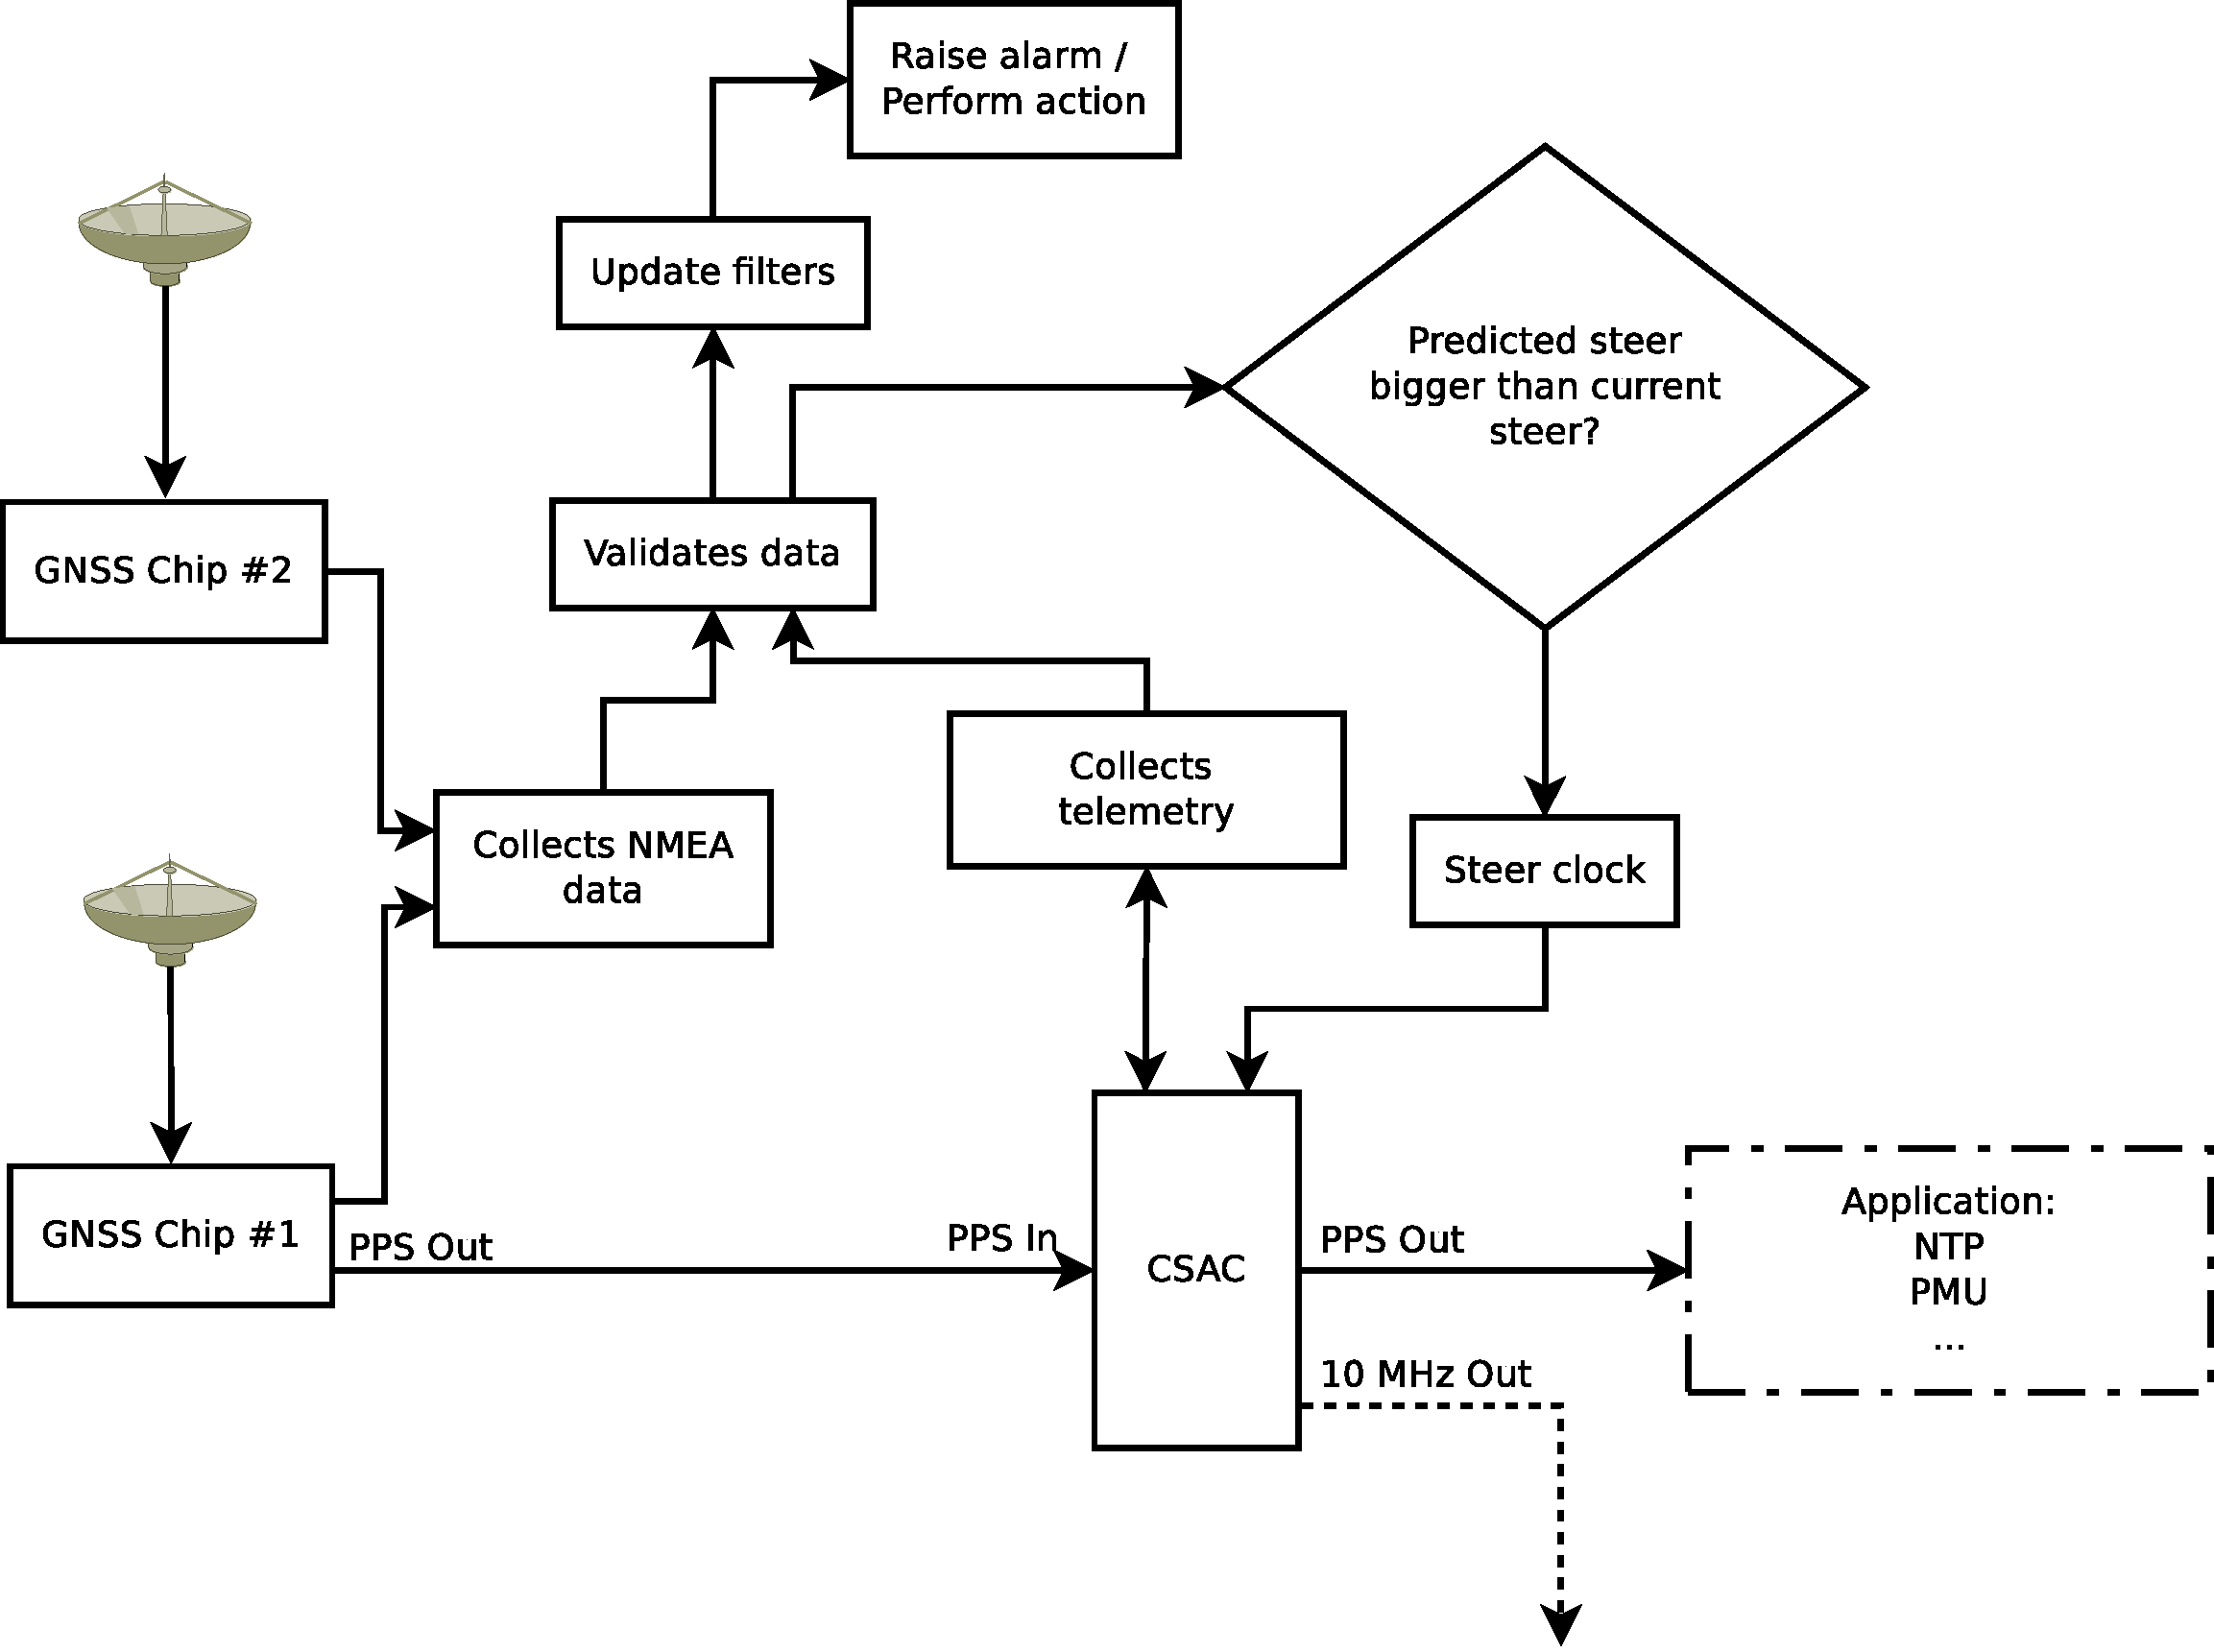
\includegraphics[scale=0.4]{master_sketch_arrows.pdf}
   \caption[atomic clock atomic clock controller Block diagram]{A block diagram of our proposed solution}
\end{figure}

\section{Implementation description}
In the following section, the architecture and inner workings, data structures and key components of the Sensor Server will be explained. The Server core (\ref{server_core}) consists of the source code in \texttt{sensor\_server.c}. The Parser and Handler spans over texttt{session.c} and texttt{actions.c}. The atomic clock model and the associated filters source code is in \texttt{csac\_filter.c}. The filter using GPS data is in \texttt{filters.c}. Figure \ref{server_call_graph} shows a simplified call graph for the Sensor Server.

\subsection{Server core}\label{server_core}
\begin{figure}
\centering
  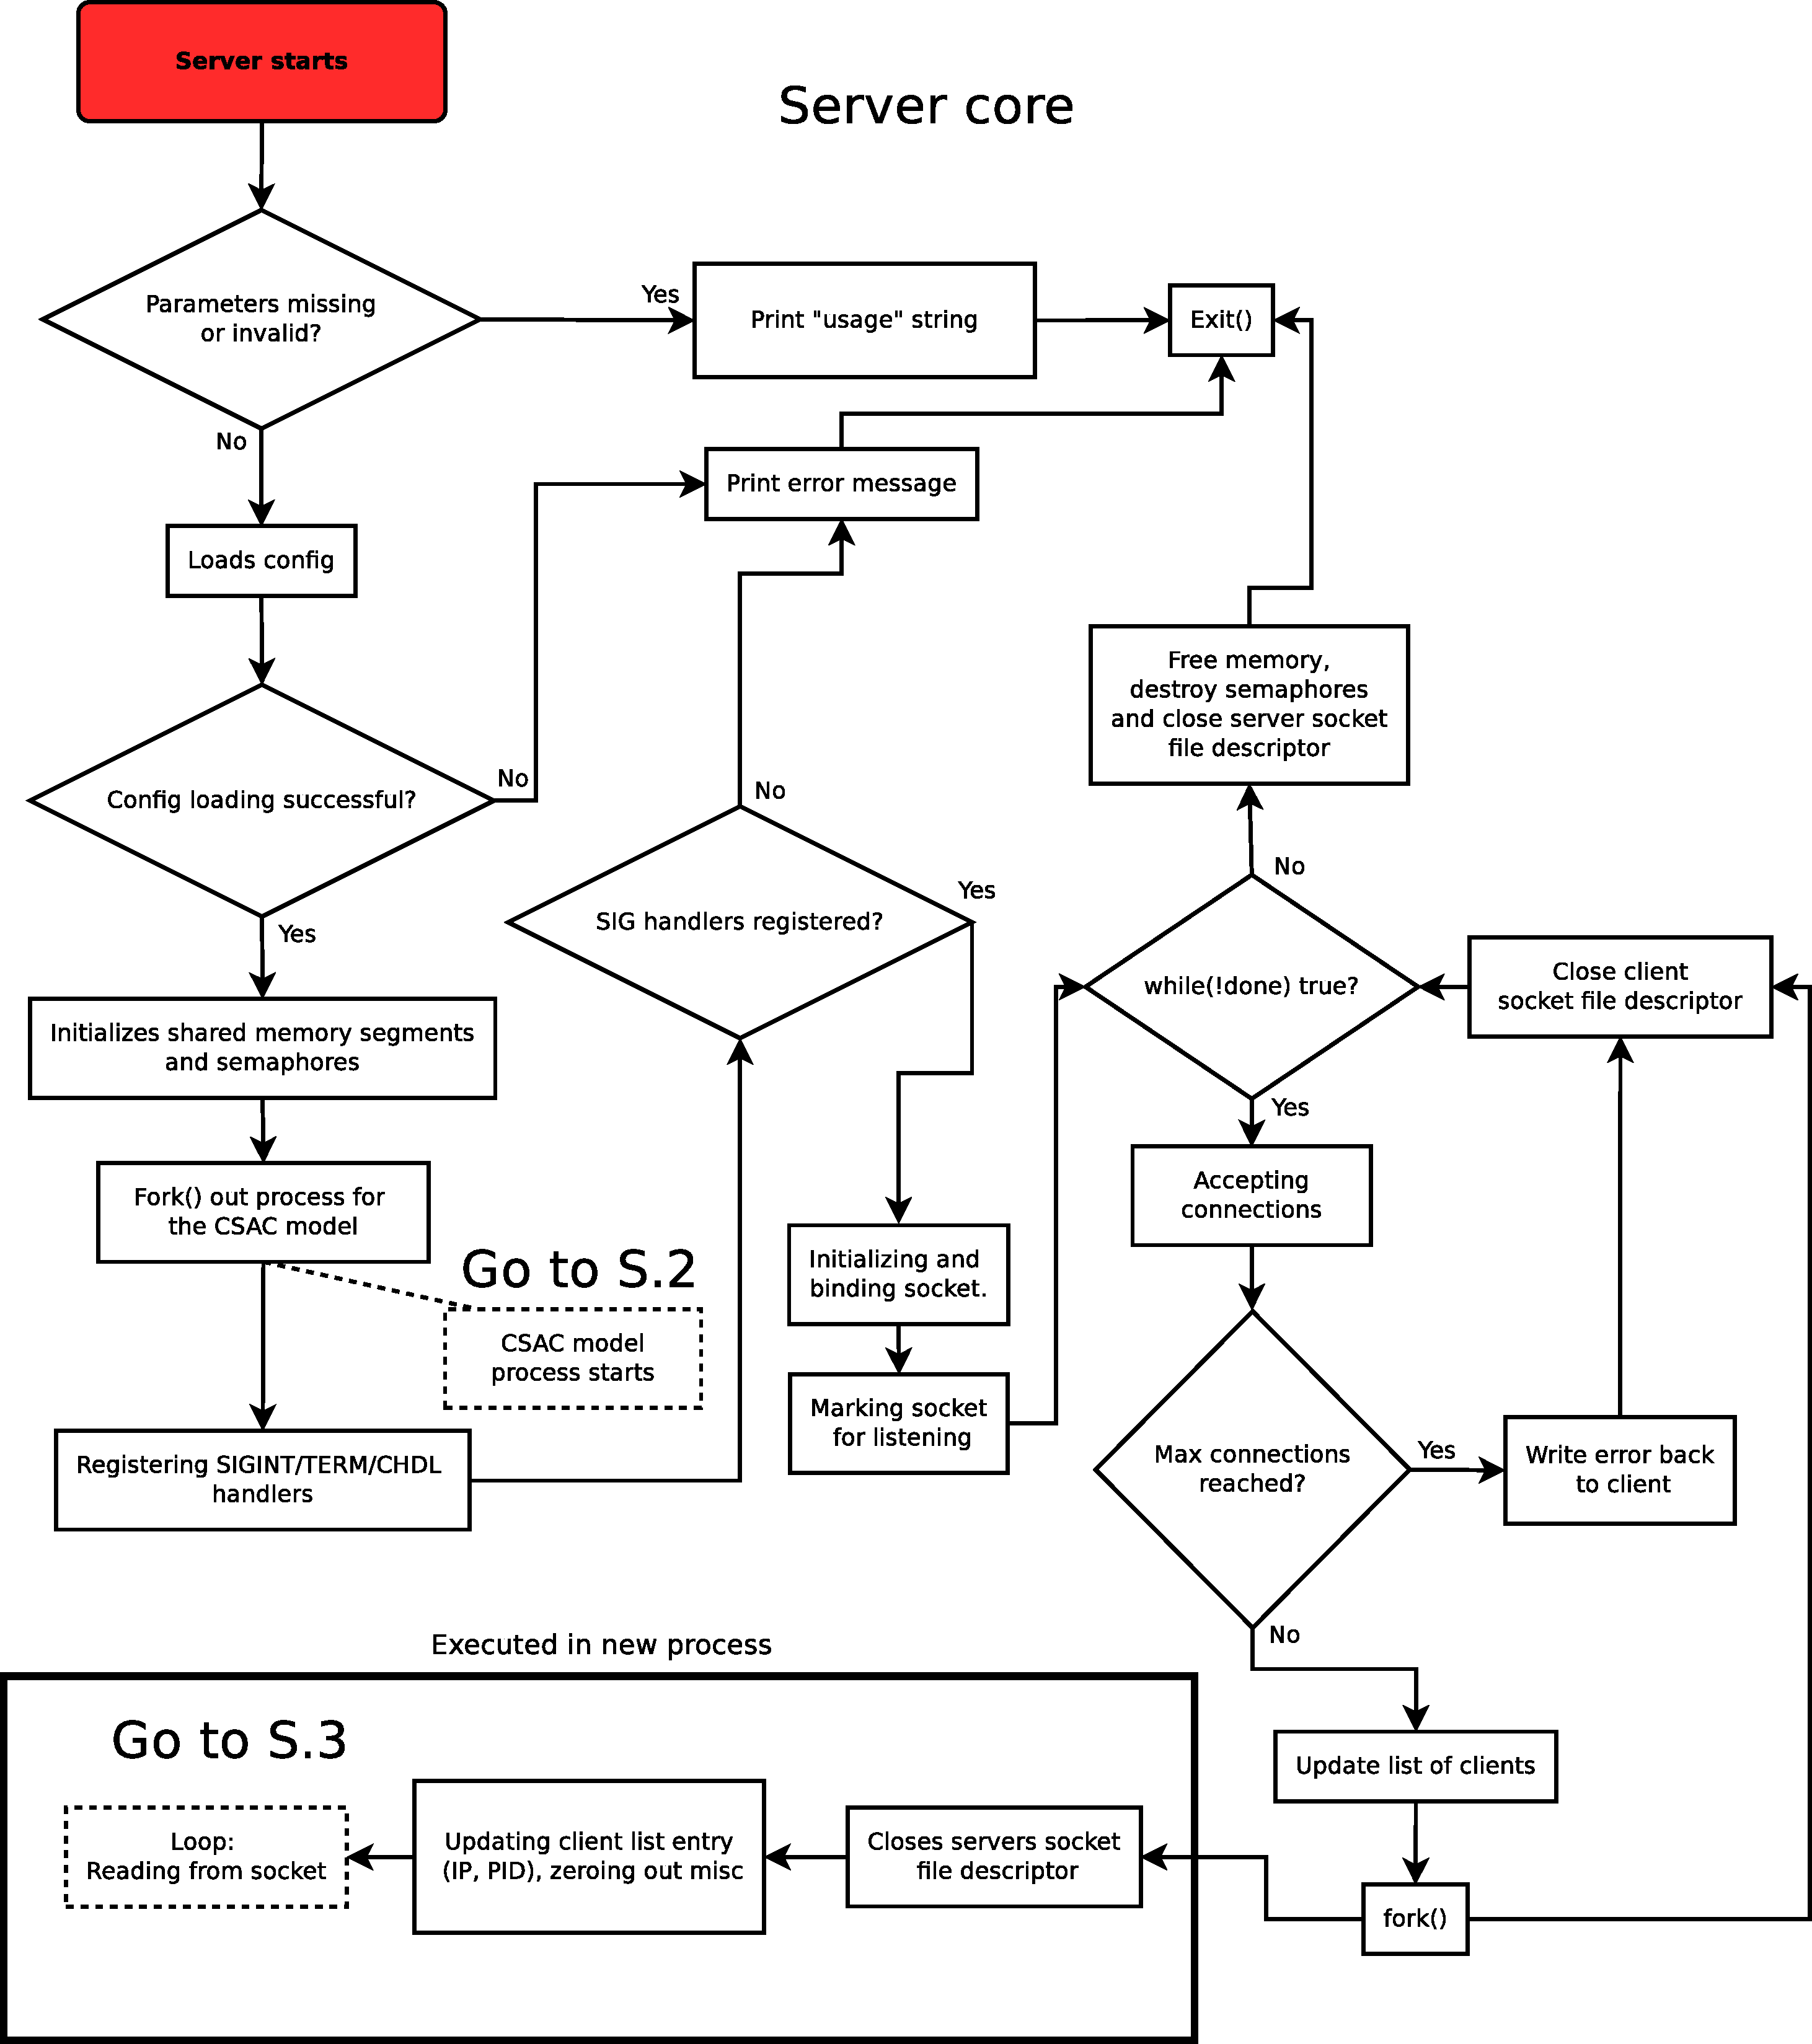
\includegraphics[scale=0.3]{server_core.pdf}
   \caption[Socket Server Core execution flow block diagram]{The block diagram shows an abstracted view of the Sensor Servers Core.}
   \label{figure_server_core}
\end{figure}

\begin{figure}
\centering
  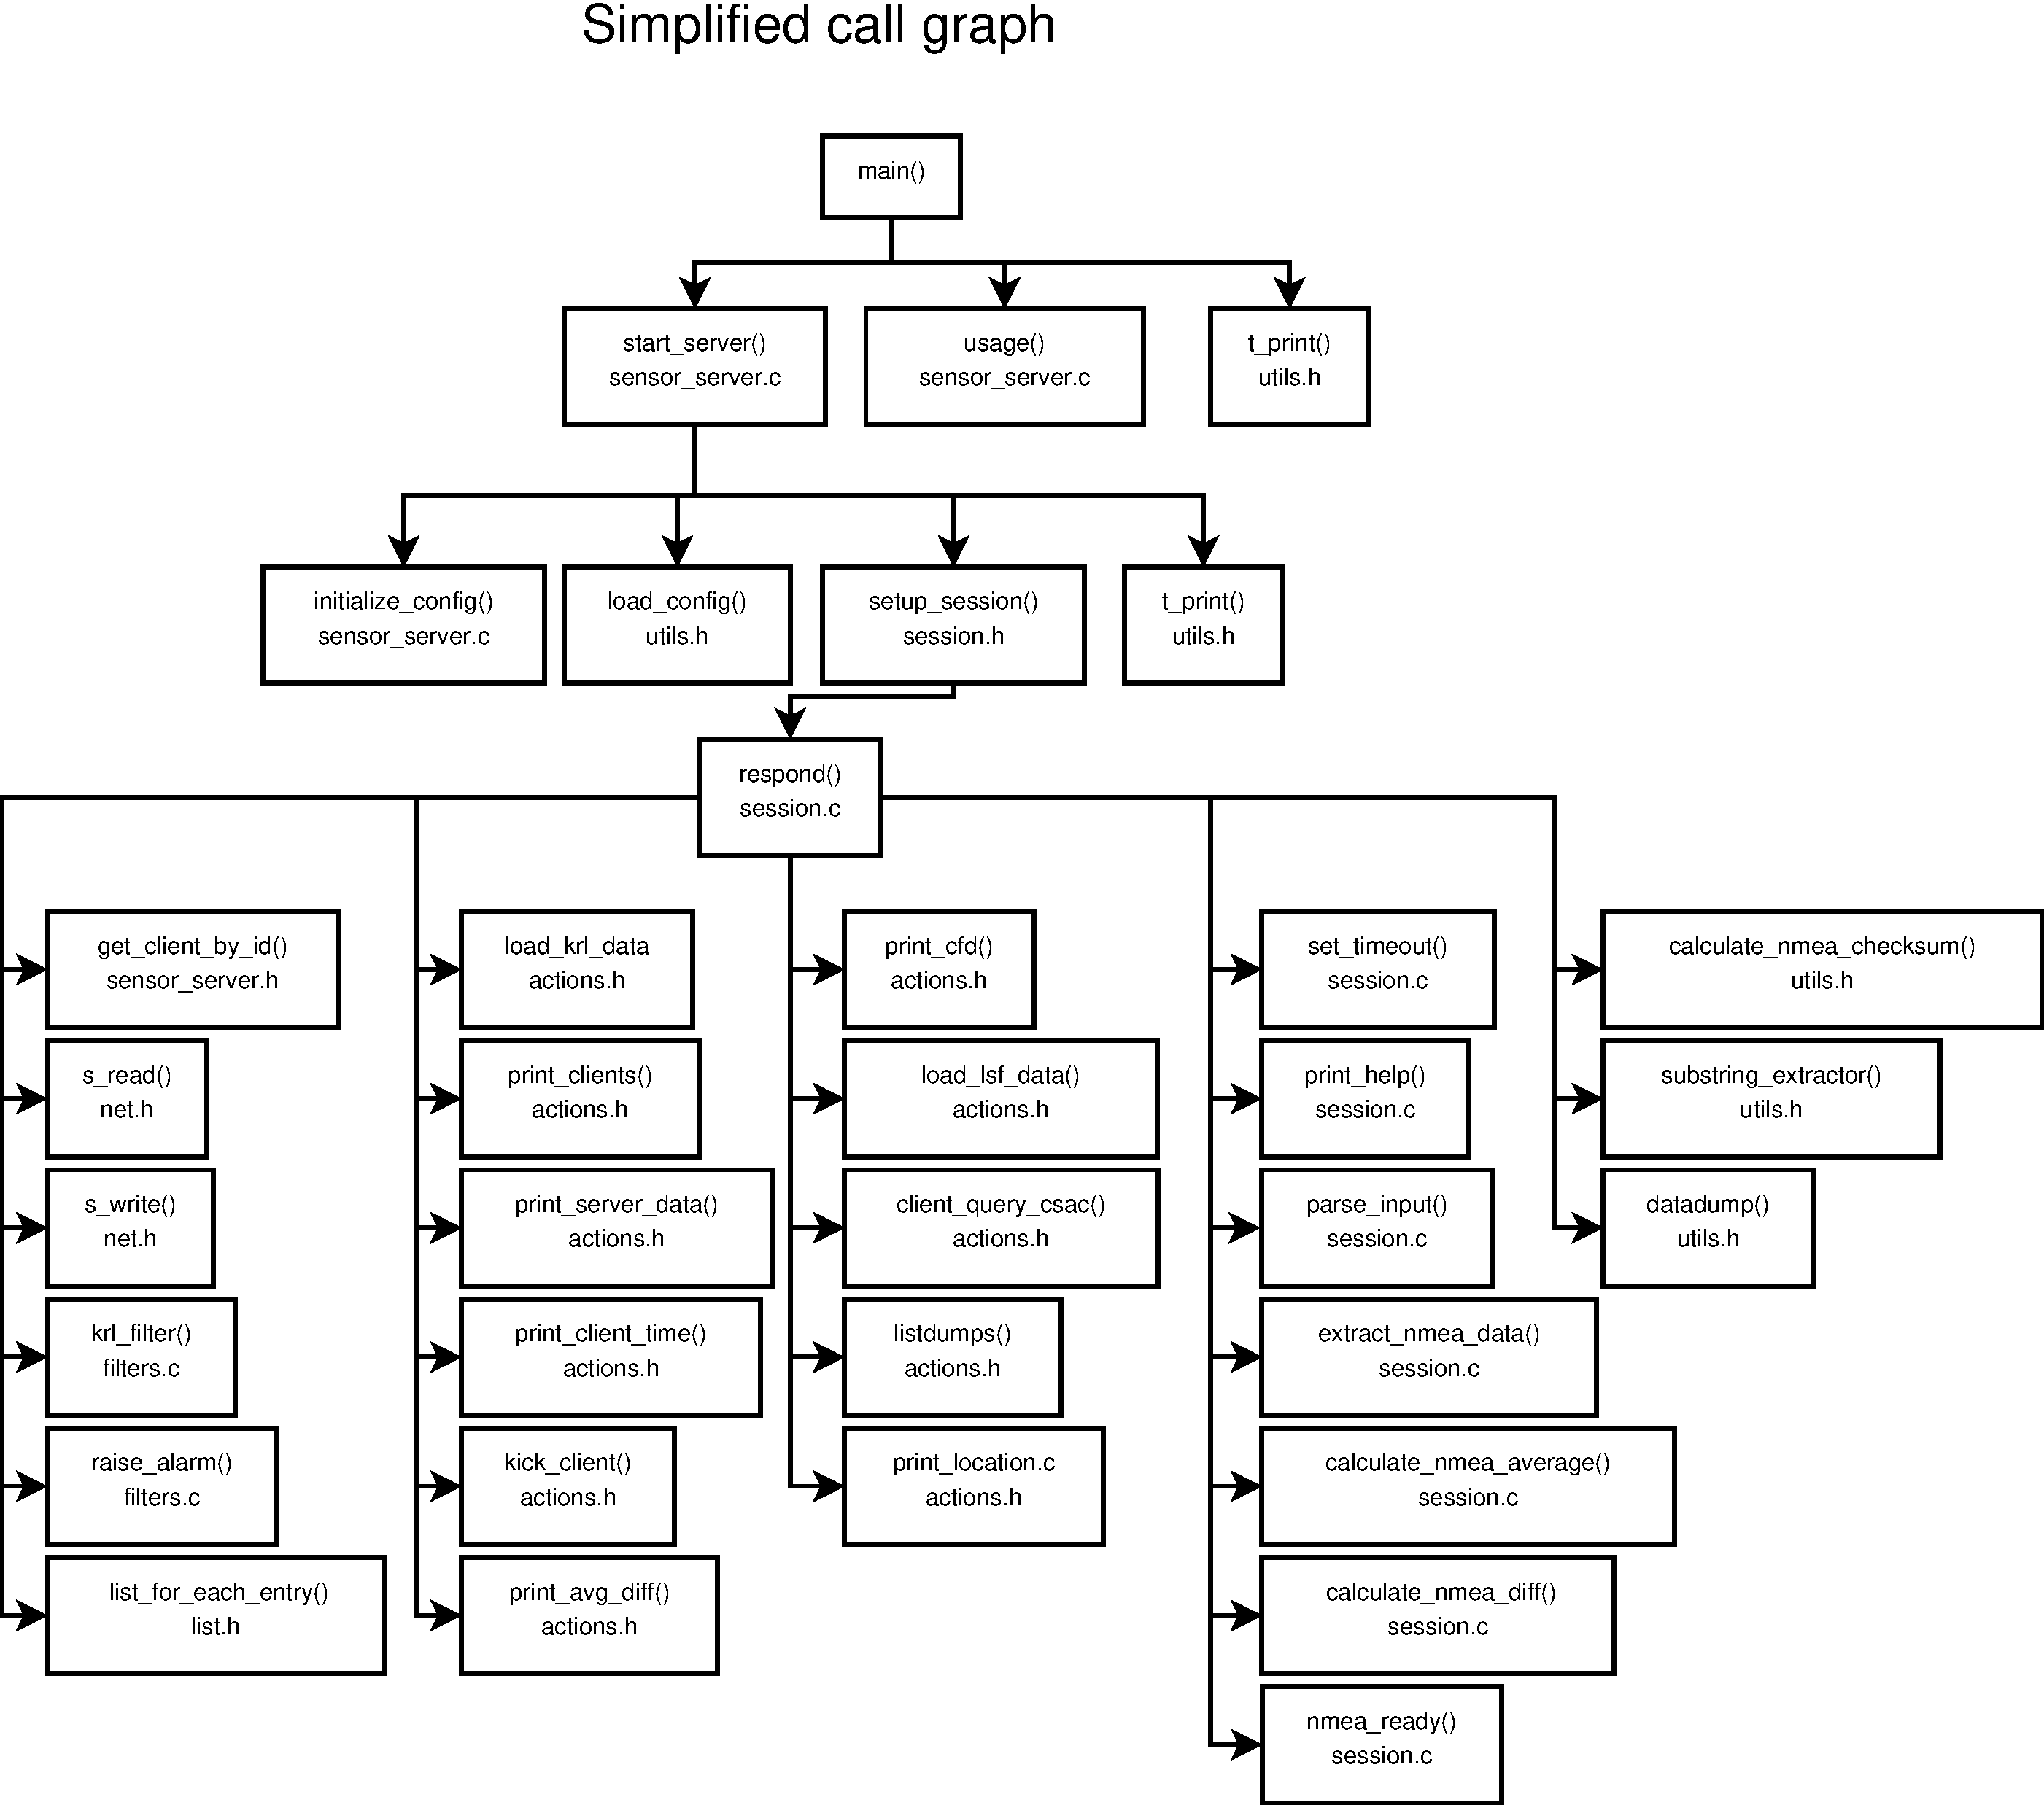
\includegraphics[scale=0.3]{server_call_graph.pdf}
   \caption[Sensor Server simplified call graph]{Simplified call graph for the Sensor Server.}
   \label{server_call_graph}
\end{figure}

The "Server core" is the main process and the parent of every process created during the life of the Sensor Server. It spawns the process maintaining the atomic clock model as well as new processes for every client that connects. Figure \ref{figure_server_core} is a block diagram of the Server core. 

\begin{itemize} % Sources needed here?
  \item The Server software takes one parameter to start, the port. If the parameter are missing or the parameter is illegal, a string containing usage information is printed and the program exits. Because the Server also is responsible for communication with the atomic clock, it needs the rights to access the serial port connected to the atomic clock \footnote{The easiest way to achieve this is to run the program as \texttt{sudo} or login as root. The best solution would probably be to add the user to a group with the right permissions. This is often the \texttt{dialout} group.}.
  \item The configuration is initialized and loaded. If the configuration fails to load, the Server prints and error message and exits.
  \item The \texttt{client\_list}, a shared memory segment containing a linked list containing all the clients, is initialized. See section \ref{clms} and \ref{linked_list} for more about the client list shared memory segment and linked list implementation.  
  \item Shared memory segments and semaphores are initialized and allocated.  If the allocation fails, the Server prints an error message and exits. See section \ref{shared_mem_sem} for more about semaphores and shared memory.
  \item The process responsible for maintaining the atomic clock model and filter s forked out. If the fork fails, the server prints an error message and exits. See section \ref{csac_model} for more about the atomic clock model.
  \item Handler for SIGINT (interrupt) SIGTERM (terminate) and SIGCHLD (child process is interrupted or terminated) is registered.
  \begin{itemize}
      \item When a process exits, a SIGCHLD signal is sent to the parent. When a client disconnects from the server, the process that handled the client exits. Ideally, the client disconnects from the server by sending a protocol compliant "disconnect request". This way, the server can handle the disconnect in a controlled manner and update its client list when the client disconnects. However, this is not always the case and if the client disconnects abruptly and without a warning, the server still needs to handle it. Therefore, when a SIGCHLD signal is received, the server iterates through its client list and finds the client who's PID matches the sender of the signal and removes it from the list. In figure \ref{server_core} this routine is the part in the red dotted box. 
  \end{itemize}
  \item The socket is initialized and marked for listening. See section \ref{sockets} for more about sockets. 
  \item A loop is entered. The loop breaks when \texttt{volatile sig\_atomic\_t done} equals 0. If the loop is broken, the semaphores are destroyed and all allocated memory is freed, the servers socket file descriptor is closed and the Server exits. See section \ref{server_synchro} for more about variables used in synchronization mechanisms.
  \item When a client connects, the server checks if the maximum number of clients has been reached. If this number has been reached, an error message is written back to the client and the clients socket file descriptor is closed. If the maximum number of clients has not yet been reached, the client list gets updated and a fork is performed.
  The parent process then resumes the loop. 
  \item The process that just forked out for the new connection, closes the server socket file descriptor it inherited from its parent.
  \item The new process then updates its client table entry and proceeds to the listening loop. This is covered in section \ref{parser_and_handler}. See section \ref{client_table_entry} for more about the client table entry struct.
\end{itemize}

\subsection{Clock model}\label{csac_model}
\begin{figure}
\centering
  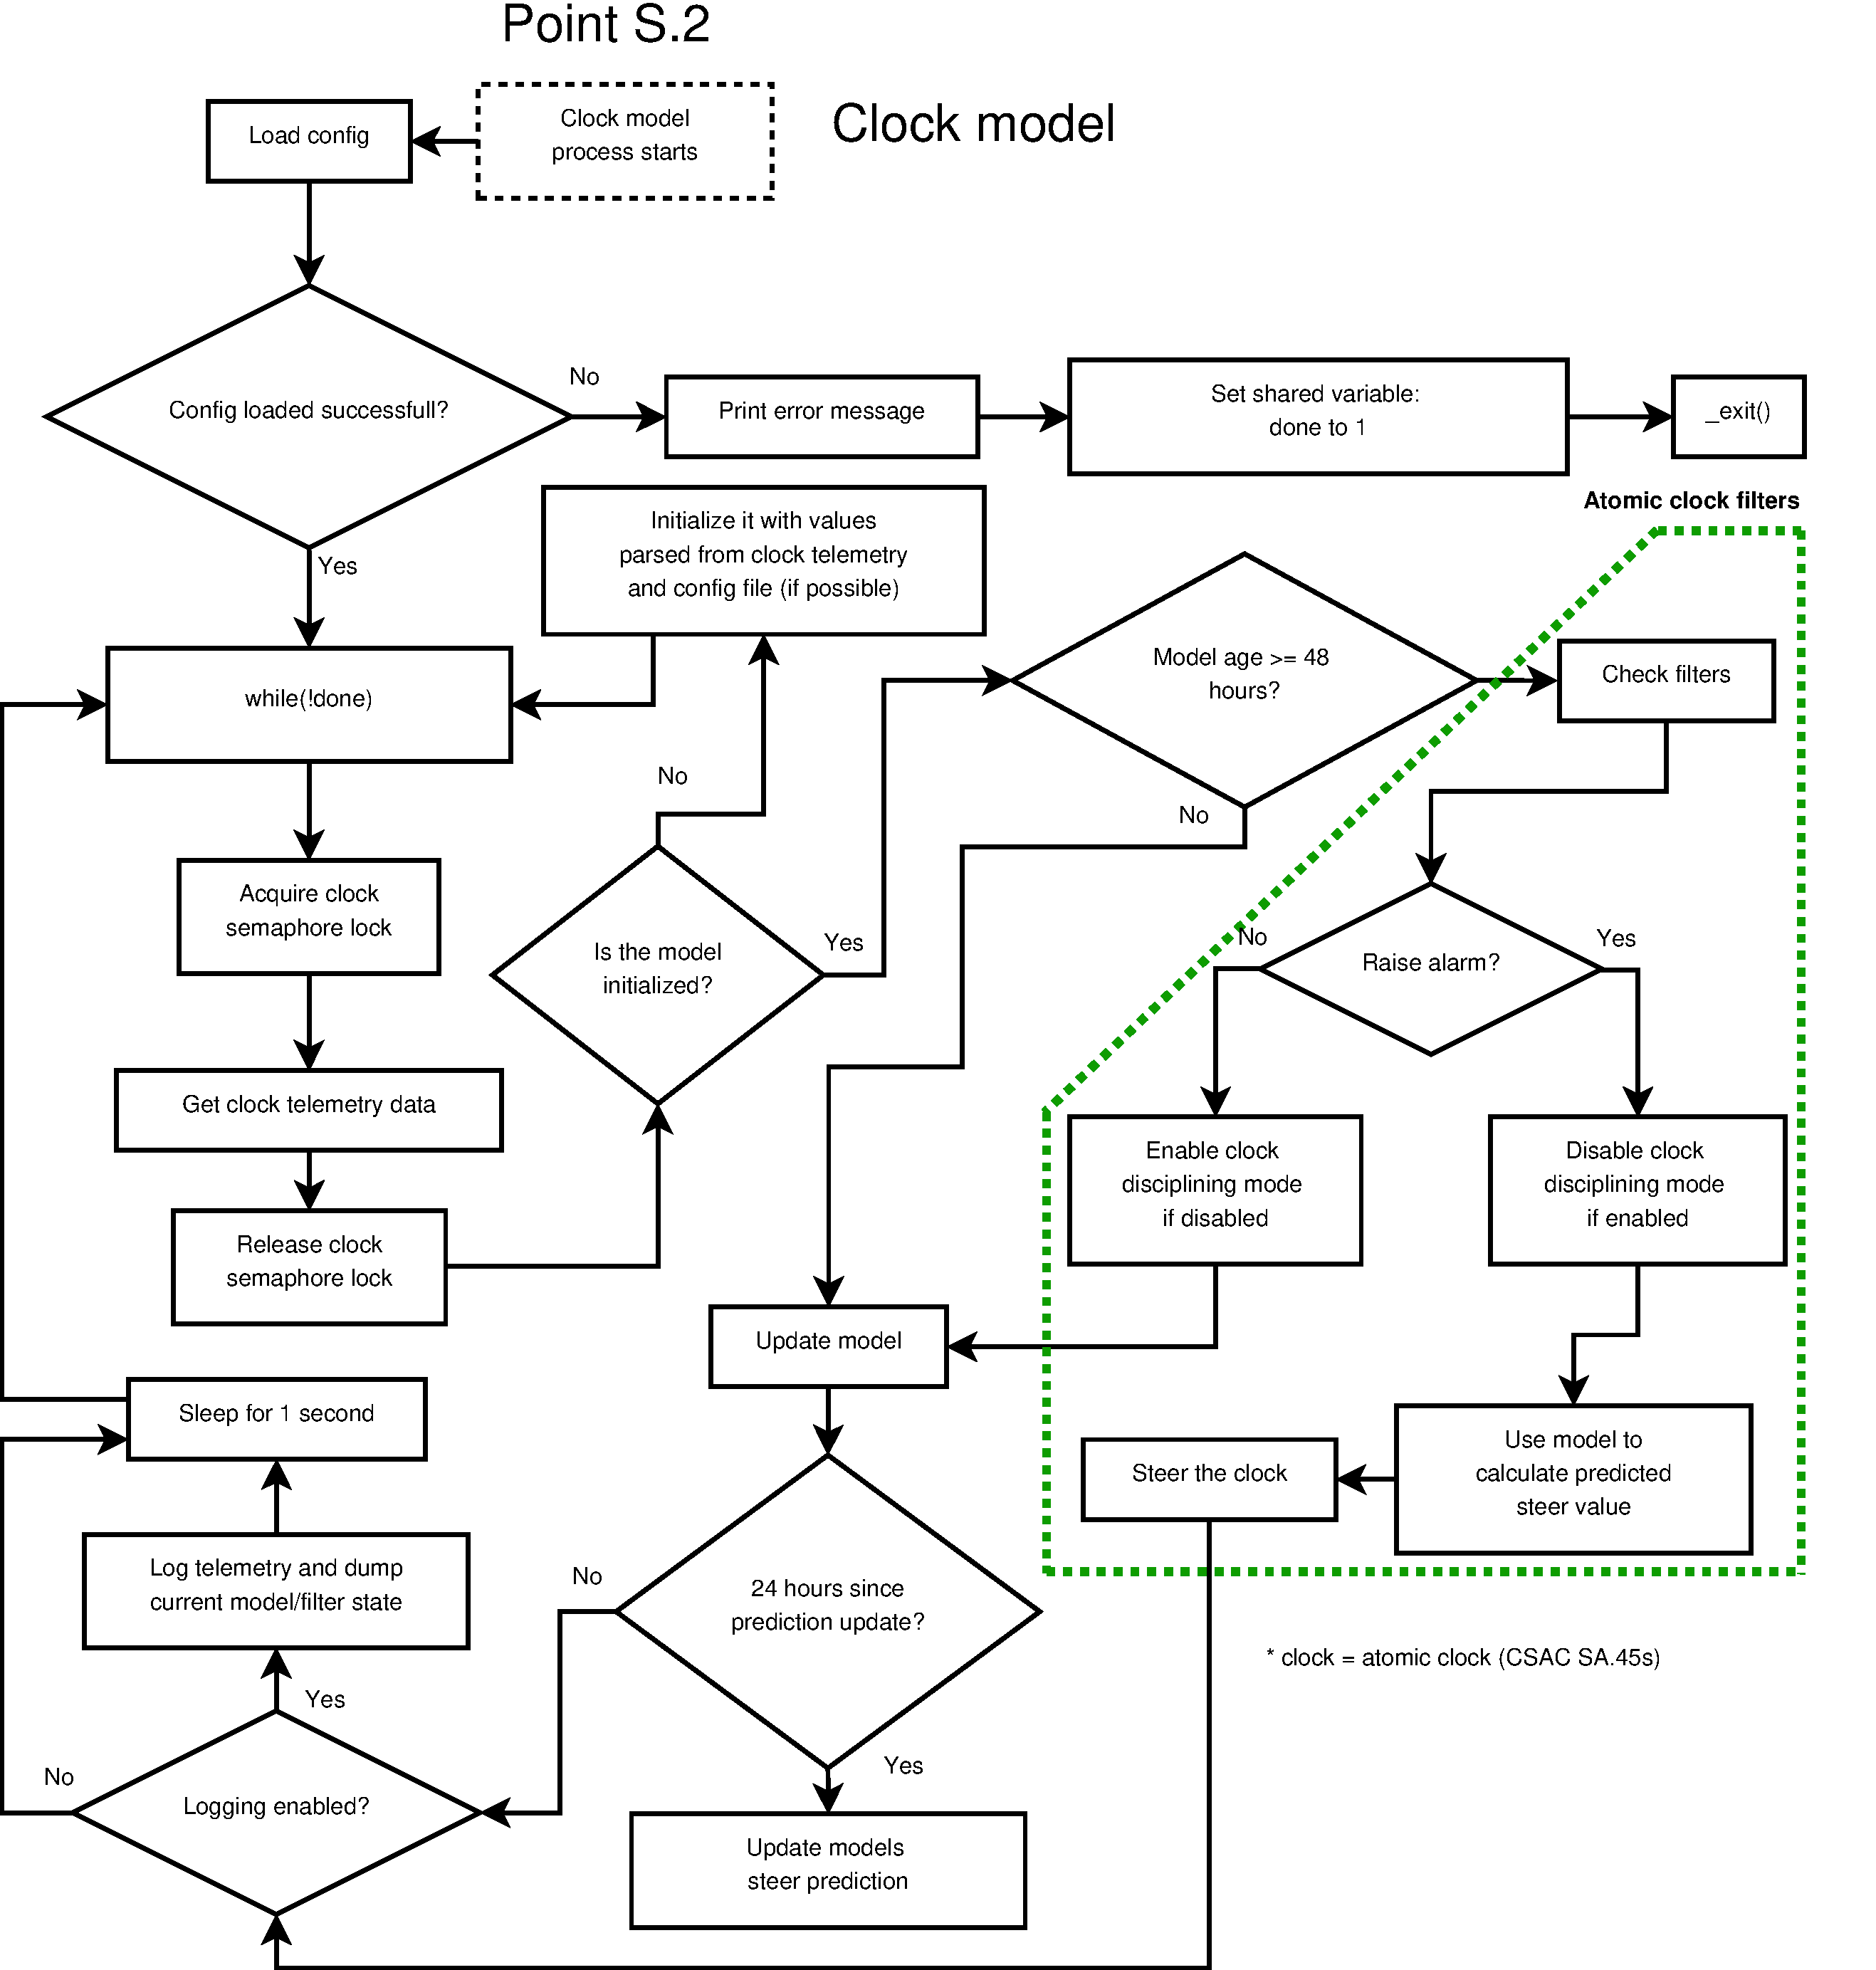
\includegraphics[scale=0.30]{csac_model.pdf}
   \caption[Execution flow the clock model]{Block diagram showing the flow of execution in the atomic clock model}
   \label{figure_csac_model}
\end{figure}
Conceptually, the atomic clock model and the filter that uses the model is two separate tasks. In practice however, they are intertwined as figure \ref{figure_csac_model} suggests. See section \ref{hw_csac} for more about the atomic clock and section \ref{csac_model_harald} for the model itself.

\begin{itemize}
  \item The configuration for the model is loaded. The configuration includes values defining the accepted limits for steering and phase difference. Optionally, it can also include state values from an "earlier" model \footnote{The functionality to restore an earlier model is not without restrictions. It is typically meant for a situation where the Server needs to be taken down for a couple hours and a new warm-up period is considered undesirable. This is better explained in section \ref{csac_model_harald}} that can be used to initialize the model further, thus reducing the warm-up time. If the loading of the configuration fails, an error message is printed, the \texttt{volatile sig\_atomic\_t done} is set to 1 and the process exits. This also breaks the server core (\ref{server_core}) loop. After all, the system needs the atomic clock to do the job it is intended for.
  \item A loop is entered. The loop breaks when \texttt{volatile sig\_atomic\_t done} equals 0. 
  \item The atomic clock lock is acquired and once the telemetry is queried from the atomic clock, it is released again.
  \item If the model is not initialized, telemetry data is used to initialize it. State values from earlier models will also be used if available in the earlier loaded configuration. See section \ref{csac_com} for more about communication with the atomic clock.
  \item A check is done to see if the model has been running for at least 48 hours. If it has, it is ready to be used a reference for the filters. See section \ref{csac_filters} for more about the atomic clock filters in particular.
  \item The telemetry received from the atomic clock is used to update the model. 
  \item A check is done to see how if 24 hours have passed since the prediction values were last calculated. The model keeps track of steer predictions for yesterday and today. By using these two points of data, an estimation of the predicted steer can be calculated. 
\end{itemize}

\subsection{Parser and Handler}\label{parser_and_handler}
\begin{sidewaysfigure}
\centering
  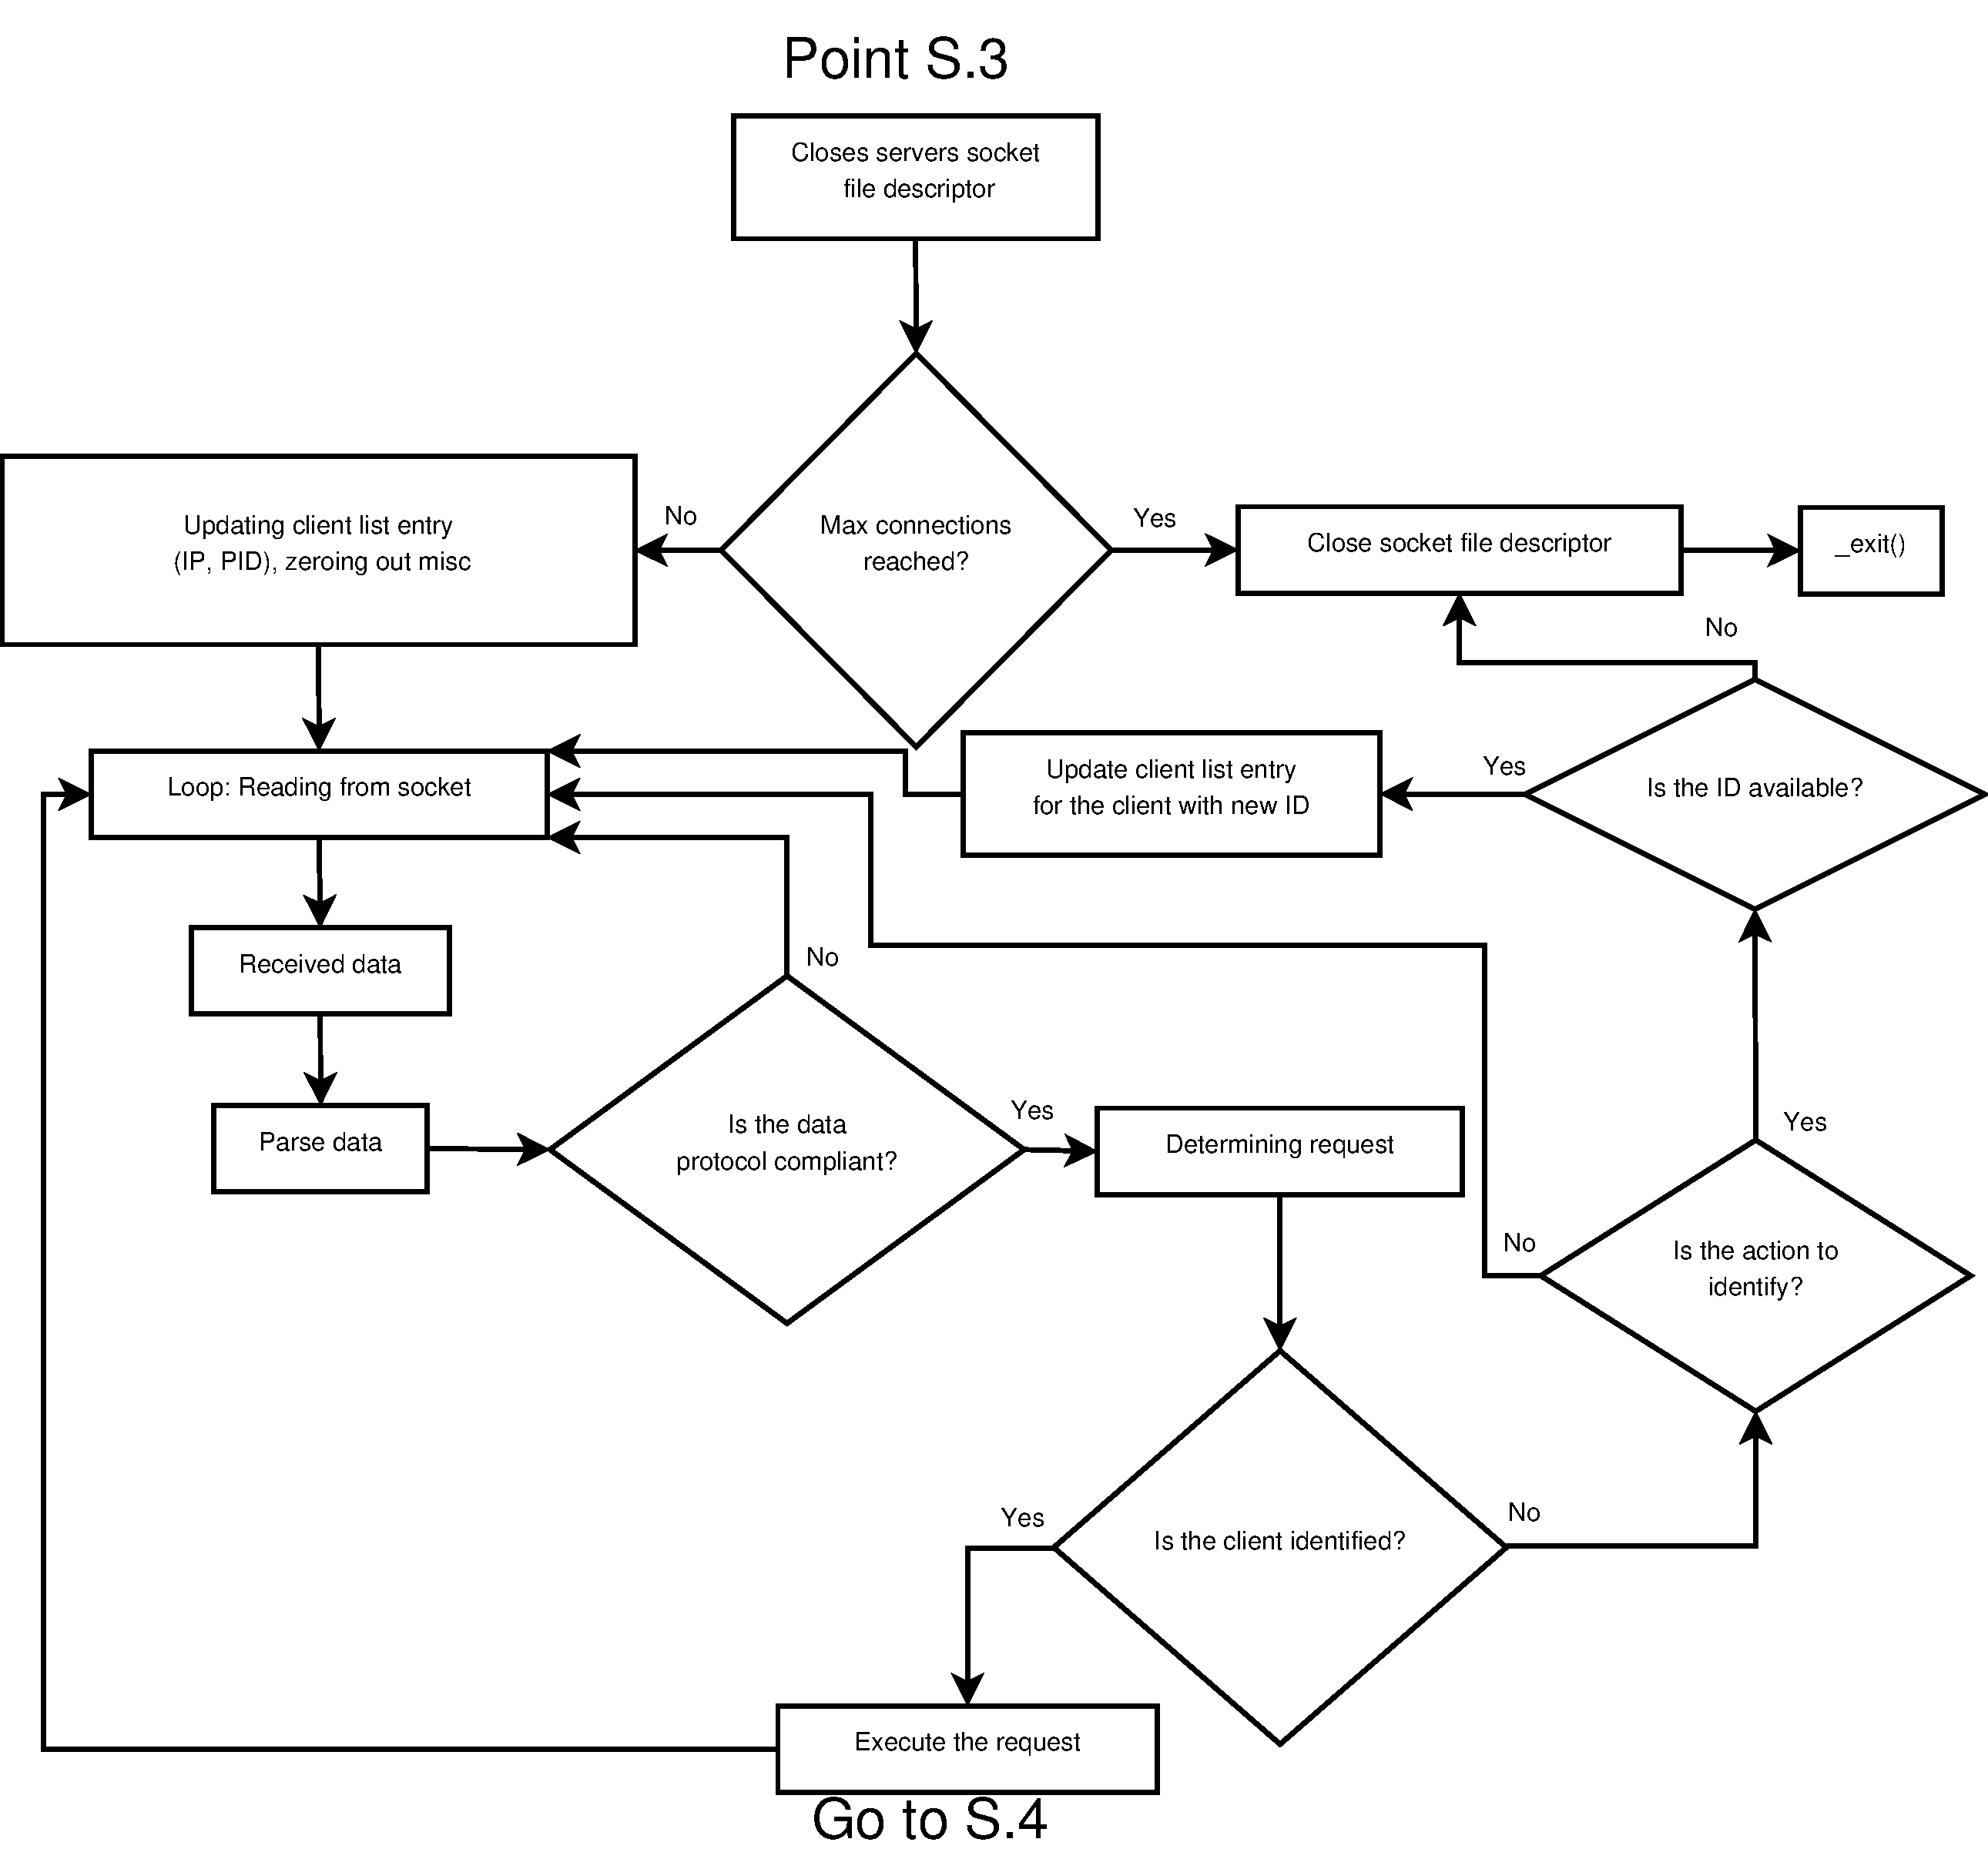
\includegraphics[scale=0.3]{server_flow.pdf}
   \caption[Socket Server execution flow block diagram]{The block diagram shows an abstracted view of execution after a client has connected to the server and a \texttt{fork()} has been performed.}
   \label{server_flow}
\end{sidewaysfigure}
\begin{figure}
\centering
  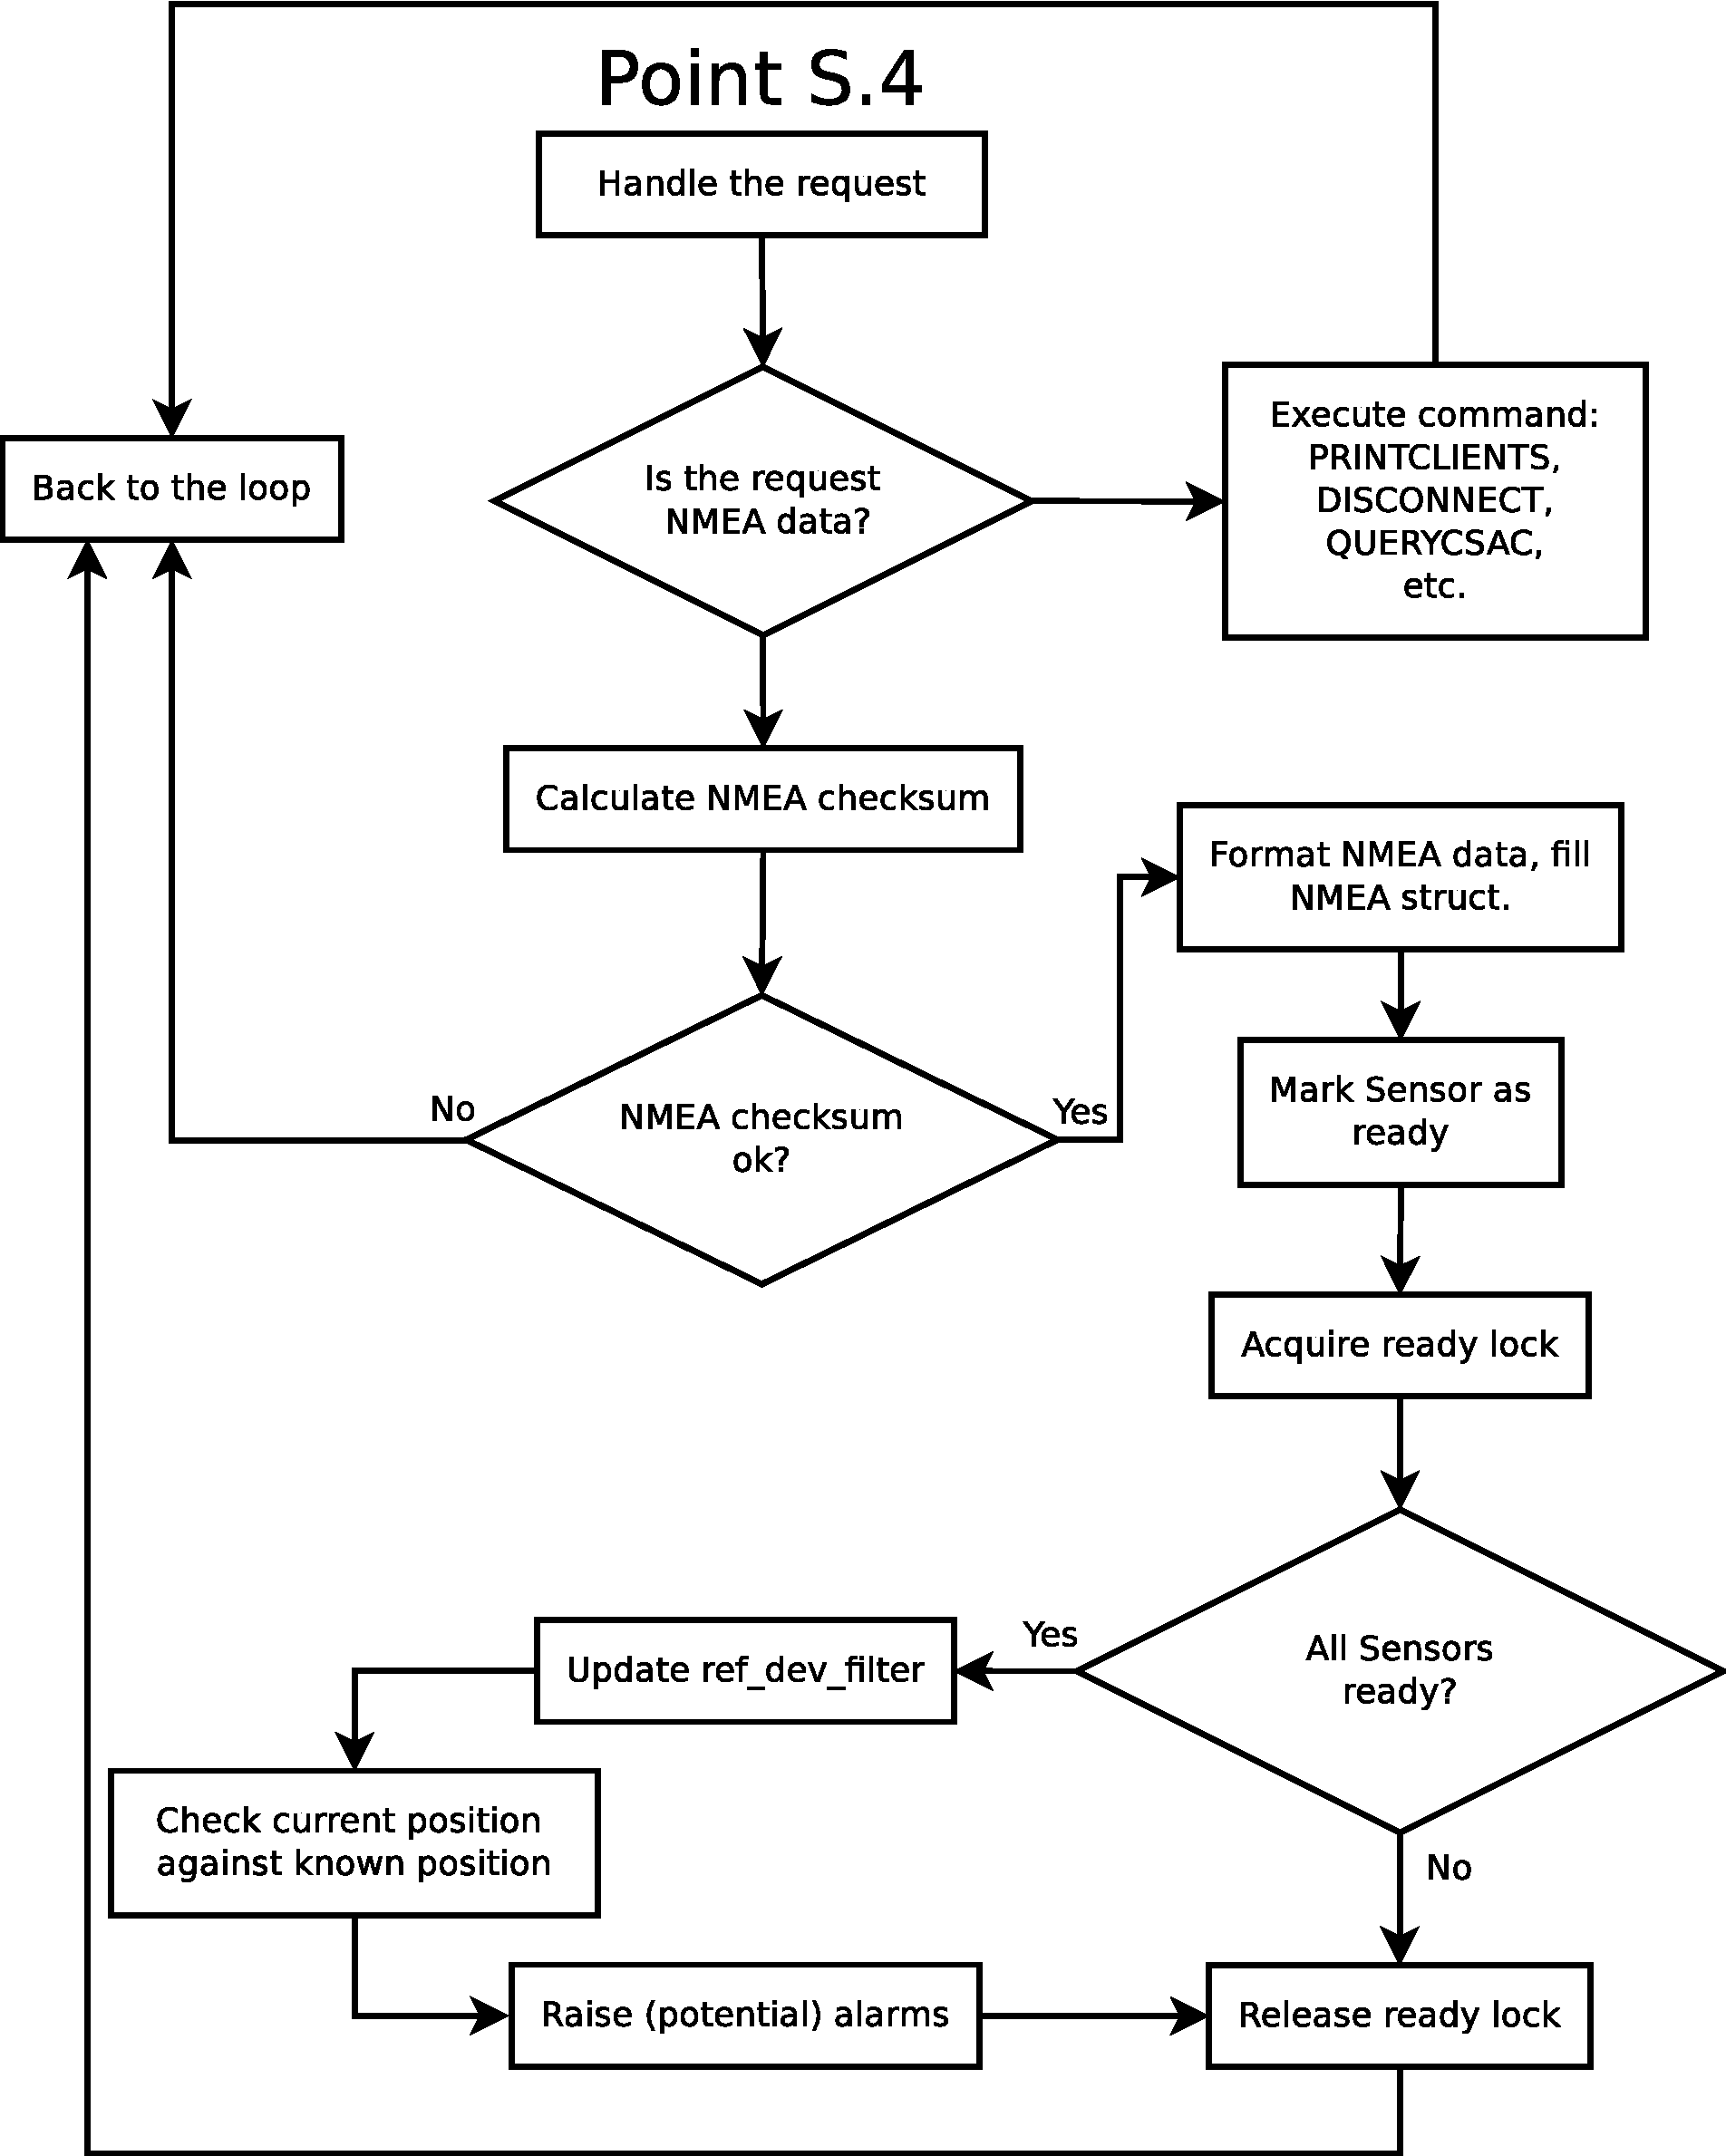
\includegraphics[scale=0.40]{actions_core.pdf}
   \caption[Socket Server execution flow block diagram]{The block diagrams shows and abstracted view of the execution after data has been received from a client.}
   \label{actions_core}
\end{figure}

The parser and handler are responsible for parsing data received from a client and making sure every request is protocol compliant. Once the goal of the request has been established, the request is executed. A function named \texttt{respond()} is called in the listening loop. Every time data is received from a client, the data is sent to the parser (\texttt{parse\_input()}) to determine the validity of the request received. See subsection \ref{nmea_data} for more information about the GPS data received from the Sensors. Figure \ref{server_flow} and \ref{actions_core} are block diagrams showing the execution flow for this part of the server. The protocol is explained in greater detail under section \ref{protocol} and the parser is better explained under subsection \ref{parser}.

\begin{itemize}
  \item A loop is entered. The loop is broken when \texttt{volatile sig\_atomic\_t done}\label{atomic_done} equals 0. This is the same variable that is used in the Server core \ref{server_core} loop and for a good reason: If the server exits, then its children should too. 
  \item If reading from the socket fails, the client gets disconnected. If it is successful, the client table entry for the connected client is checked to see if the client has been marked to be kicked. If it is, it gets disconnected. 
  \item The data received from the client is parsed and checked against the protocol. If the request received from the client doesn't match any of the supported requests or commands, the request is ignored and the loop is entered again. See section \ref{protocol} for more information about the protocol and subsection \ref{parser} for more information about the parser.
  \item If the request received is valid, the clients ID is checked to determine whether or not it has identified itself. If the client has identified itself, the request gets carried out. 
  \item If the request received is to handle NMEA data, the checksum for that NMEA data is calculated. If the checksum check fails, the data is discarded. If it succeeds, the data is copied into \texttt{nmea\_container} struct (\ref{nmea_cont}) for easier handling.
  \item The client is marked as ready for processing and a ready check is commenced. The ready check is used to make sure that all the sensors have received NMEA data and are ready to have filters applied. Once the filters have been applied, the lock is released and normal execution resumes. The ready check is explained further under subsection \ref{ready_check_alg}.
  \item If the clients ID is 0, it is considered unidentified and any other requests but to identify itself, is ignored.
  \item If the client is attempting to identify itself, the ID it attempts to use is checked against the rest of the connected clients. If the ID is already taken and the client attempted to assume the role of a Sensor, the client will get disconnected. If it attempted to assume the role of a Monitor, it will simply be notified that the chosen ID is taken and the request will be ignored. The reason why a Sensor would get disconnected and a monitor would not, is simple: When connecting the Sensor to the server, it should not be any doubt whether or not it has been accepted. If something is wrong, it is better that a user of the system has to deal with it there and then and configure the Sensor correct rather than allowing the user to do mistakes that severely impacts the efficiency of the system. See section \ref{roles} for more information about the Sensor and Monitor roles.
  \item If the attempted ID is available, the client table entry for the client is updated with the requested ID and the server will attempt to load data for the Location and speed filter (LS) data into the clients LS filter struct. The server will attempt to load this data from a file named \texttt{krl\_data\_sensor<ID>}. If the load fails, the client will be disconnected. It is after all useless without its reference position data. For more information about LS filter, see section \ref{kvsrlf}.
\end{itemize}


\subsection{GPS filter}\label{gps_filters}
There is currently only one filter using GPS data in the Sensor Server implementation to this data. This is the \textit{Location and speed filter}. Figure \ref{gps_filters} is a block diagram showing the filter as a part of the Sensor Server.

\subsubsection{Location and speed filter}
\begin{figure}
\centering
  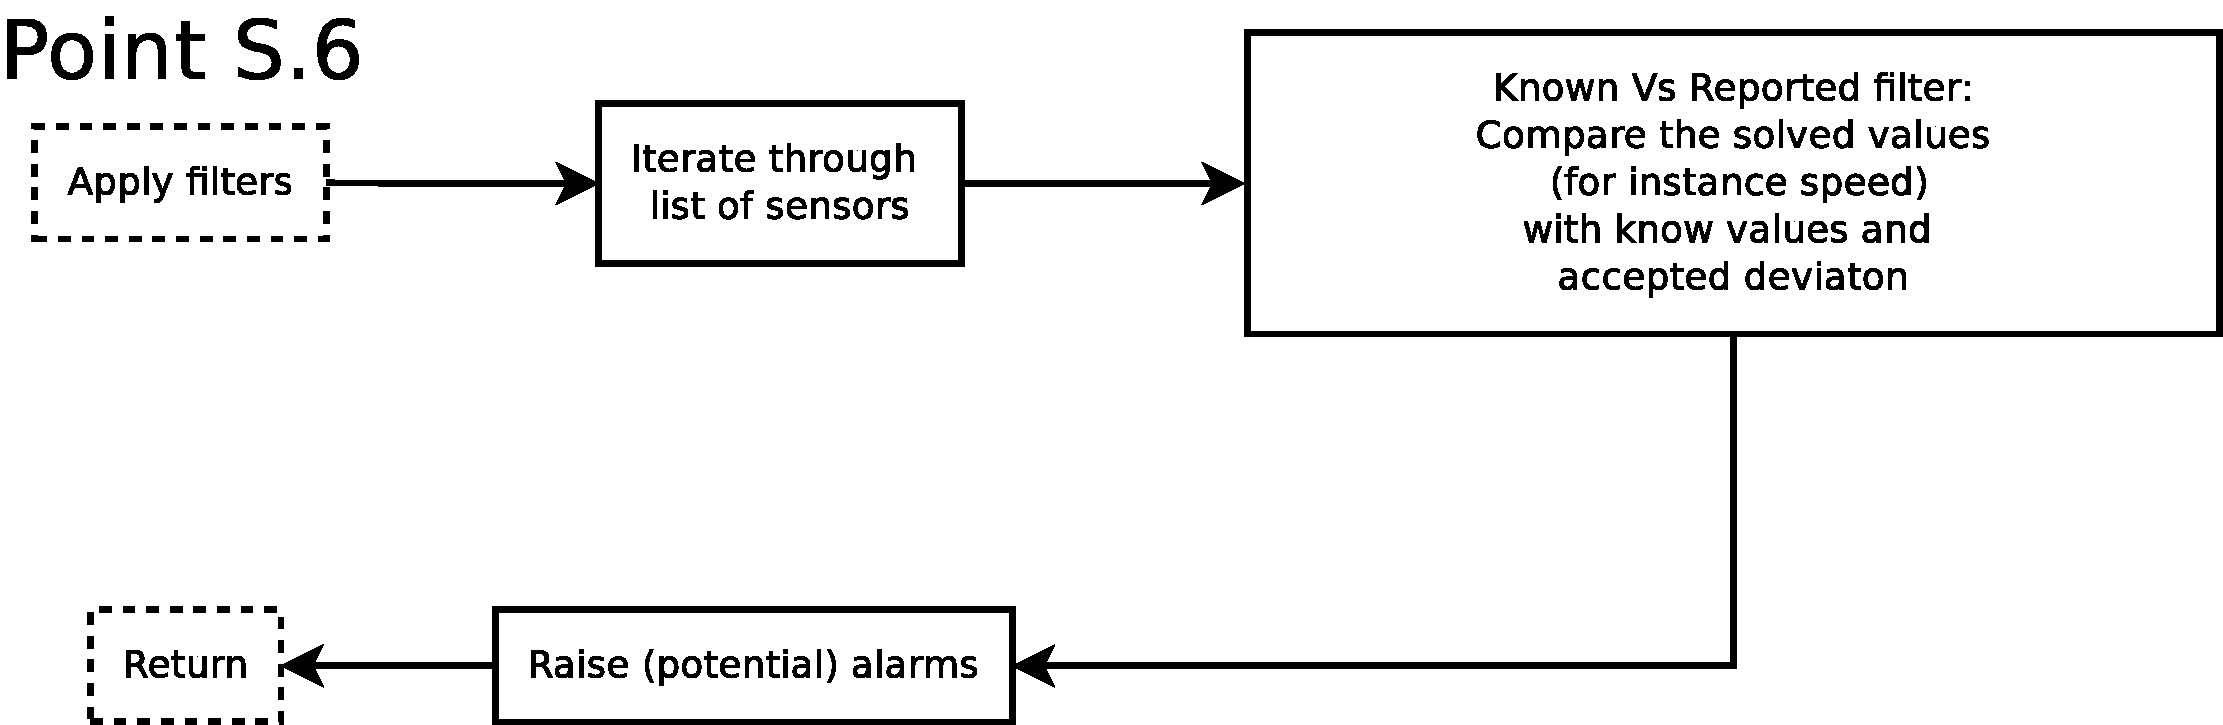
\includegraphics[scale=0.3]{filters.pdf}
   \caption[Order of execution in the filter]{Block diagram show the order of execution in the GPS filter(s)}
   \label{gps_filters}
\end{figure}
By configuring the Sensor Server with the location of the different Sensors, the server can trigger an action if a Sensor reports an abnormal solved position. The filter is triggered when either latitude, longitude, altitude or speed is higher or lower than the reference value minus or plus a deviation. Listing (\ref{ref_dev_filter_latitude}) shows an edited sample of code taken from \texttt{filters.c}. The code in the sample is part of the algorithm used to check whether or not the latitude part of the GPS receivers solved position is within "safe" (not spoofed) range.
\begin{code}
  \caption{Listing shows sample of code taken from \texttt{filters.c} line 79. The code is part of the algorithm that compares the known position of a Sensor with the Sensor resolved position. The code has been edited for clarity.}
    \begin{minted}
    [
      fontsize=\footnotesize,
      fontfamily=tt,
      linenos=true
    ]
    {c}
        if(latitude_current > latitude_reference + latitude_deviation) {
            moved = 1;
            lat_disturbed = HIGH;
        } else if(latitude_current < latitude_ref - latitude_dev) {
            moved = 1;
            latitude_disturbed = LOW;
        } else {
            latitude_disturbed = SAFE;
        }
    \end{minted}
    \label{ref_dev_filter_latitude}
\end{code}

When a Sensor connects to the Server and identifies itself, the Server will attempt to load a file containing the location of the Sensor as well as the accepted deviation values for the solved position. Listing \ref{krl_config} shows an example of such a file.

\begin{code}
  \caption{Location and speed filter configuration file}
    \begin{minted}
    [
    fontsize=\footnotesize,
    fontfamily=tt,
    linenos=true
    ]
    {c}
    alt_ref: 123.8
    lon_ref: 1102.1948
    lat_ref: 5958.5448
    speed_ref: 0
    alt_dev: 10
    lon_dev: 0.005
    lat_dev: 0.005
    speed_dev: 10
    \end{minted}
    \label{krl_config}
\end{code}

\subsection{Clock model filters}\label{csac_filters}
Figure \ref{figure_csac_model} shows both the atomic clock model and filter in one figure. As explained in section \ref{csac_model}, the model of the atomic clock and the filters based upon, are closely related. 
\begin{itemize}
  \item Once the model has been running for a configurable long time (48 hours was used during testing, see \ref{clock_model_harald} for more about the model), it is ready to be used as a reference, filtering out abnormal data.
  \item The filters are checked. There are currently three filters implemented using the atomic clock model as reference:
  \begin{itemize}
    \item \textit{Fast timing filter}. This is a simple filter that compares the current phase reported by the atomic clock with a pre-configured limit. If the current phase is higher, the filter is triggered.
    \item \textit{Frequency correction filter}. This is a more sophisticated filter. It uses the atomic clock model to calculate a predicted steer value and compares it to the current steer value. If the current steer is too big, the filter is triggered. 
  \end{itemize}
  \item If any of the filters are triggered, the alarm is raised. The state of the alarm is expressed by an \texttt{int} that is either 0 or 1. If the alarm was not raised, the disciplining of the atomic clock is enabled if it was disabled, and the telemetry data is used to update the model.
  \item If the alarm is raised, the disciplining of the atomic clock is deactivating, thus protecting the atomic clock from being affected by the spoofing. The model is now used to calculate steer values that are applied to the atomic clock instead.
\end{itemize}

\subsection{GPS data}\label{nmea_data}
The GPS receivers that we have chosen for our system and possibly all GPS receivers, follow the National Marine Electronics Association's 0183 standard \cite{NMEA_MAIN}. NMEA data consists of sentences where the first word of the sentence, the type, defines how the sentence should be interpreted. The sentences used by the Sensor Server and Client, is the \texttt{GNRMC} for latitude, longitude and speed and \texttt{GNGGA} for altitude.  

\subsection{Client connection}\label{sockets}
Every time a client connects to the server, a process is forked for the new connection. Listing \ref{server_connect} is sample of code taken from the core of the Sensor Server, and can be explained like this:
\begin{itemize}
  \item Line 4: The server waits for a connection. \texttt{accept()} is a blocking function. The code does not continue past this point before a client has connected.  
  \item Line 12: A client has connected. The server creates a new process to handle the new connection. The new process is created using \texttt{fork()}.
  \item Line 13: Both the new process and its parent enters the if statements regarding its process identification (PID). The parent does not match the criteria of the ifs and returns to the top of the loop. The child on the other hand, matches the criteria for the if sentence at line 15.
  \item Line 16: The child process closes it's parent's socket file descriptor and continues to setup the session at the next line.
\end{itemize}
\begin{code}
  \caption{Sample of code taken from \texttt{sensor\_server.c}(\ref{sensor_server.c}, line 494). The sample has been edited for clarity purposes.}
  \begin{minted}
  [
  fontsize=\footnotesize,
  fontfamily=tt,
  linenos=true
  ]
  {c}
    listen(server_sockfd,SOMAXCONN);
    int session_fd = 0;
    while (!done) {
        session_fd = accept(server_sockfd,0,0);
        if (session_fd==-1) {
            if (errno==EINTR) continue;
            t_print(ERROR_CONNECTION_ACCEPT,errno);
        }
        if(number_of_clients == max_clients) {
            close(session_fd);
        } else {
            pid_t pid=fork();
            if (pid==-1) {
                printf(ERROR_FAILED_FORK, errno);
            } else if (pid==0) {
                close(server_sockfd);
                setup_session(session_fd, new_client);
                close(session_fd);
                _exit(0);
            } else {
                close(session_fd);
            }
        }
    }
  \end{minted}
  \label{server_connect}
\end{code} 

\subsection{Shared memory \& Semaphores}\label{shared_mem_sem}
The architecture uses several shared memory segments. The pointers to the shared memory segments are declared as \textit{extern} in \texttt{sensor\_server.h}. The extern keyword means the the variable has an external linkage, making it visible from other files than the one in which it is defined. Listing \ref{extern_structs} shows a code sample taken from \texttt{sensor\_server.h} where the shared memory segments are declared.
\begin{code}
  \caption{Sample of code from \texttt{sensor\_server.h}(\ref{sensor_server.h}, line 44) where shared memory segments are declared.}
  \begin{minted}
  [
  fontsize=\footnotesize,
  fontfamily=tt,
  linenos=true
  ]
  {c}
    extern struct client_table_entry *client_list;
    extern struct server_data *s_data;
    extern struct server_synchro *s_synch;
    extern struct server_config *s_conf;
    extern struct csac_filter_data *cfd;
  \end{minted}
  \label{extern_structs}
\end{code}

These shared memory segments have different usage. The \texttt{client\_list} points to a shared segment allocated for storing a list of all connected clients. \texttt{s\_data} contains information about the server, \texttt{s\_synch} contains semaphores used to lock down shared resources, \texttt{s\_conf} is the servers configuration and \texttt{cfd} is the data and state for the filters based on the clock model. Every process that forks out from the server is given access to these memory segment. One might make the point that this voids the idea of processes, and one might be correct (see \ref{discussion}). The shared memory is created using the GNU library's Memory Mapped I/O (MMAP). Although typically used to map files to a region of memory, MMAP can also be used to create an anonymous map which is not connected to file but rather for sharing data between tasks without using files. Listing \ref{mmap_use} shows an example of MMAP being used to map an anonymous, shared map for the client list.

\begin{code}
  \caption{Listing shows the use of MMAP to create an anonymous map of memory to be used as a shared memory segment. Sample of code taken from \texttt{sensor\_server.c}(appendix \ref{sensor_server.c}, line 360)}
  \begin{minted}
  [
  fontsize=\footnotesize,
  fontfamily=tt,
  linenos=true
  ]
  {c}
  client_list = mmap(NULL, 
                    (s_conf->max_clients * sizeof(struct client_table_entry)), 
                    PROT_READ | PROT_WRITE,
                    MAP_SHARED | MAP_ANONYMOUS | MAP_NORESERVE,
                    -1, 0);
  \end{minted}
  \label{mmap_use}
\end{code}

\subsection{Client list memory segment}\label{clms}
Every time a client connects, it is given a piece of shared memory where it can store its data. This piece of shared memory is used as a node in a linked list. The linked list structure, stored in the shared memory segment is available to all the processes spawned by the server. This segment is static in size and is allocated once and is never changed during the whole life of the Server. The size of the segment is determined by the maximum number of allowed clients, a configurable value read from the configuration file every time the server is started. Read more about why the client list shared segment is static in size, under subsection \ref{resizing_shared}. 

\subsubsection{Using the client list memory segment}\label{create_client}
As previously explained, the list of clients are stored in a shared memory segment using a linked list structure. In order to keep tabs on what part of the shared memory segment is in use, a simple map of the memory is used (\ref{memory_map_figure}):
\begin{figure}
\centering
  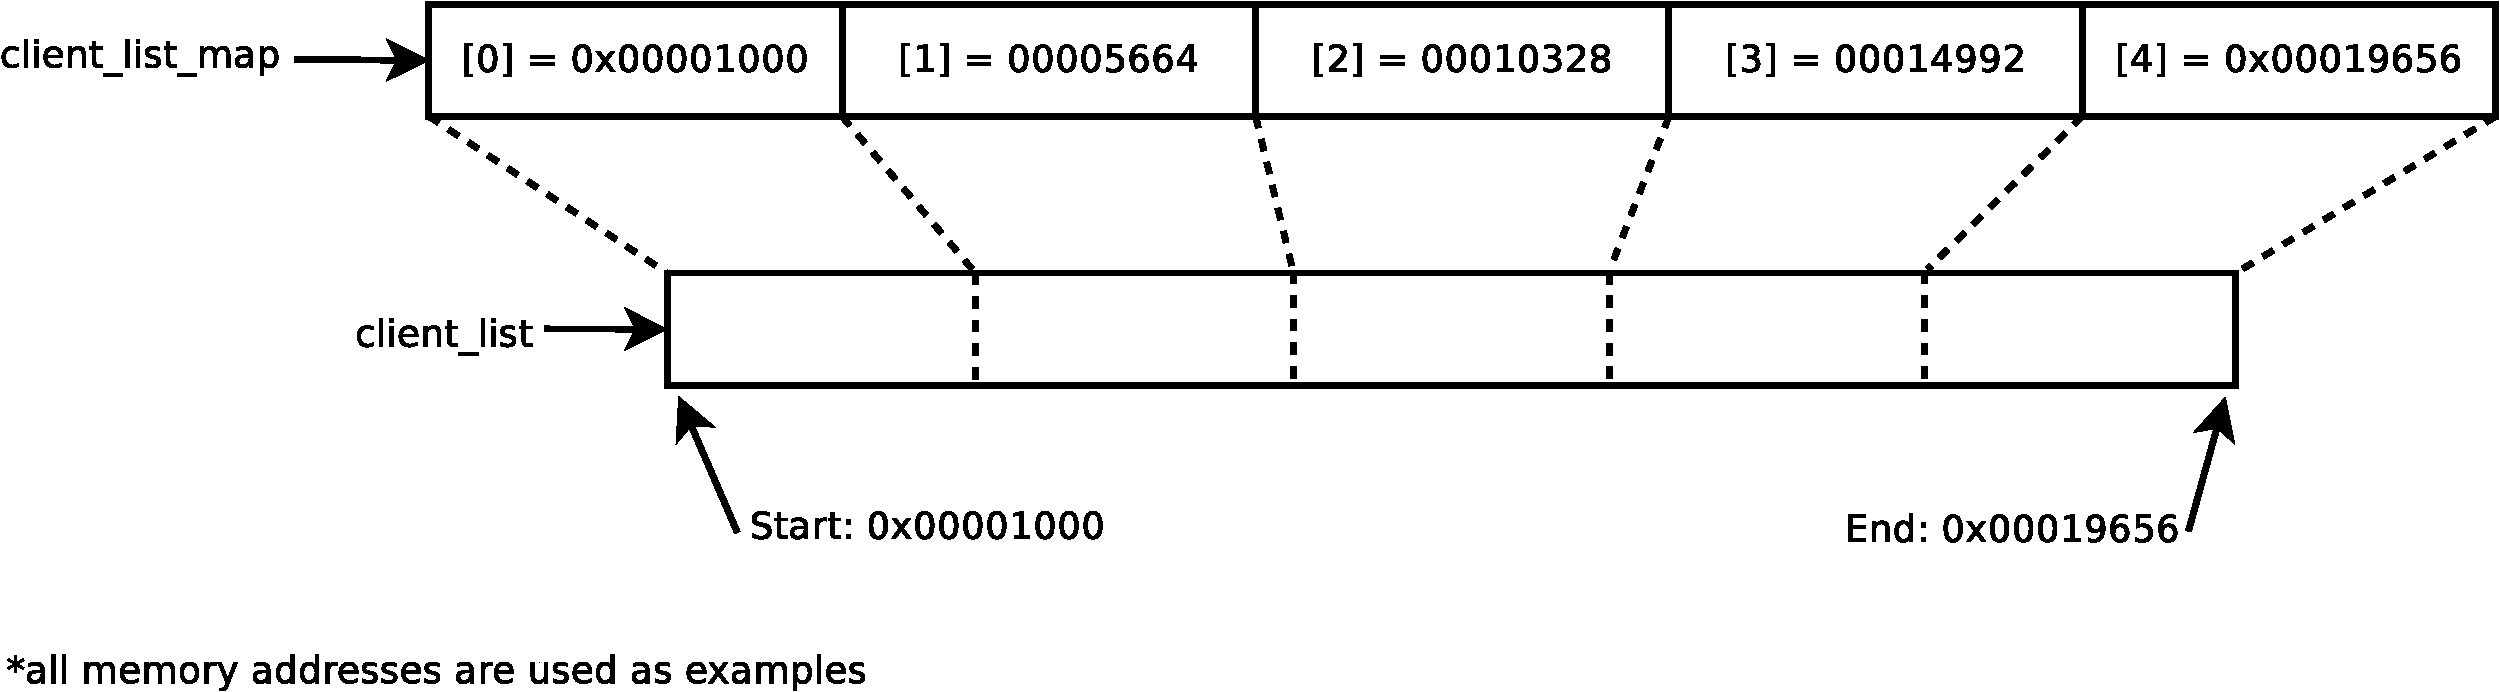
\includegraphics[scale=0.3]{mem_layout.pdf}
   \caption[Memory map layout example]{Figure is showing the relation between the shared memory segment containing the client list and the memory map}
   \label{memory_map_figure}
\end{figure} 

The map is an array containing pointers to the client list segment. These pointers are offset by the size of the \texttt{client\_table\_struct} and maps 1:1 to what can be thought of as individual \textit{pieces} of memory in the client list shared memory segment. A free piece of memory is in the map represented by a pointer that is not NULL. Figure \ref{memory_map_null_figure} is an illustration showing the state of the map when four of the first pieces have been given out. Listing \ref{get_mem_piece} shows the function that iterates through the map to find a free piece. 

\begin{figure}
\centering
  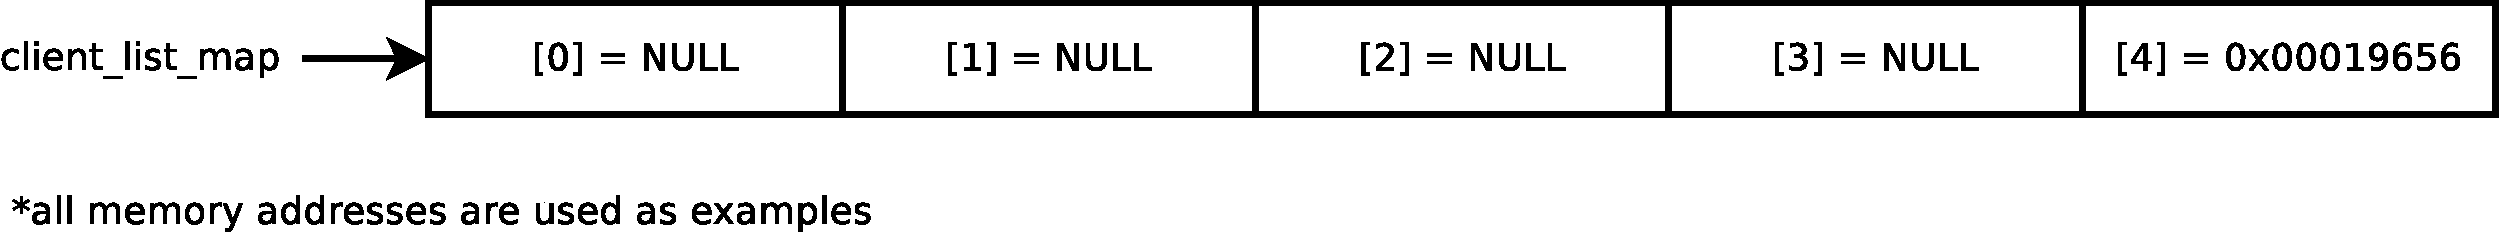
\includegraphics[scale=0.3]{mem_layout_nulls.pdf}
   \caption[Memory map layout example]{Figure is showing the relation between the shared memory segment containing the client list and the memory map after some of the pieces of shared memory has been given out.}
   \label{memory_map_null_figure}
\end{figure}

\begin{code}
  \caption{Sample of code showing the \texttt{get\_mem\_piece()} function. This function is used to find a free piece of memory in the client list shared memory segment. The code is taken from line 200 in \texttt{sensor\_server.c} (appendix \ref{sensor_server.c}}
    \begin{minted}
    [
    fontsize=\footnotesize,
    fontfamily=tt,
    linenos=true
    ]
    {c}
    static struct client_table_entry* get_mem_piece()
    {
        int i;
        for(i = 1; i < s_conf->max_clients; i++){
            if(client_list_map[i] != NULL){
                struct client_table_entry *tmp = client_list_map[i];
                client_list_map[i] = NULL;
                return tmp;
            }
            i++;
        }
        return NULL;
    }
    \end{minted}
    \label{get_mem_piece}
\end{code}

\subsection{Client linked list}\label{linked_list}
Since the C standard does not provide data structures like linked lists, I had to choose between reinventing the wheel or finding some implementation to drop into the project. While studying another subject, I found a guide on how to use the linked list implementation from the linux kernel source code (\cite{KAZU_LIST}) in a user space program. Since the implementation was solid, well tested and had many useful functions, i decided to use it. The modified header file containing all the code, is GPL licensed.  
Figure (\ref{linked_list_figure}) shows pieces of the shared memory segment linked together in a linked list structure.

\begin{figure}
\centering
  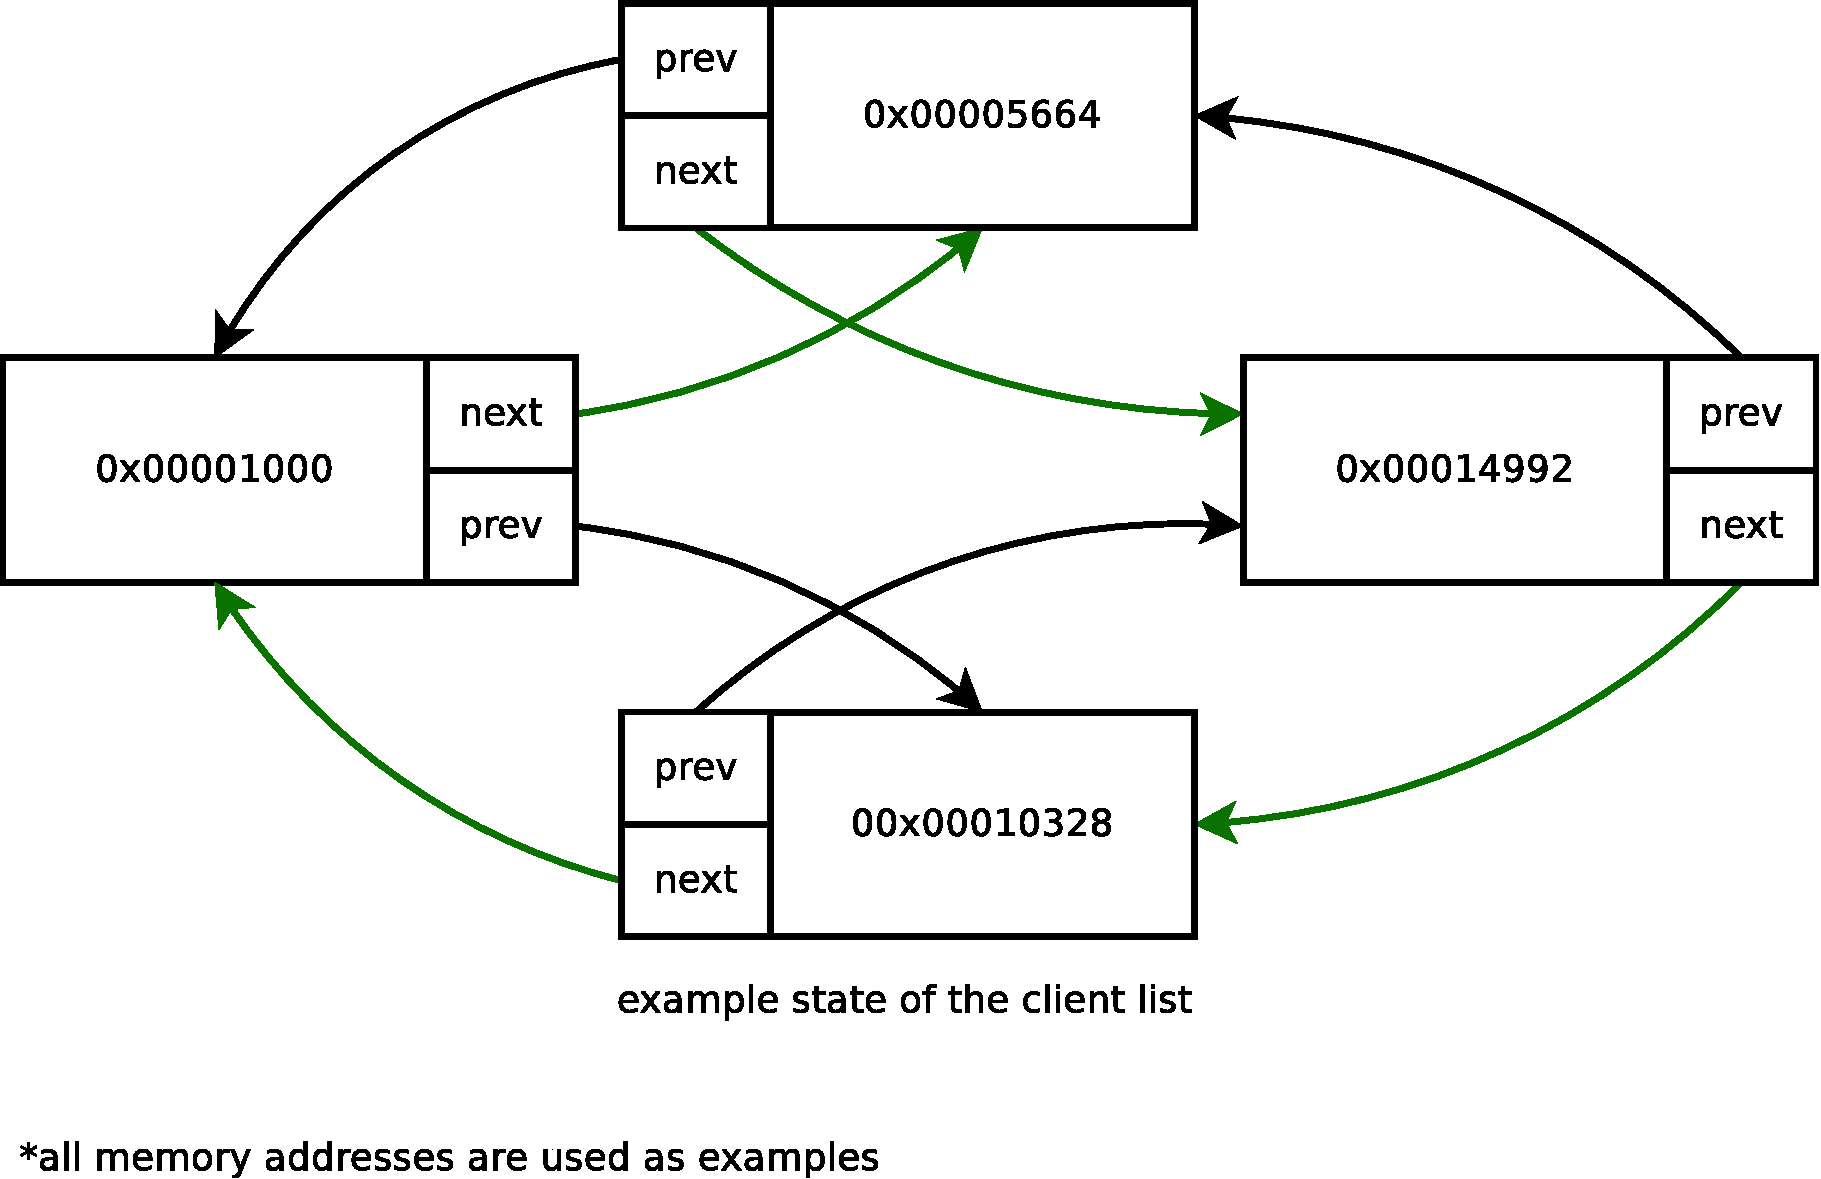
\includegraphics[scale=0.3]{linked_list.pdf}
   \caption[Linked list example]{Block diagram show an example of linked list state}
   \label{linked_list_figure}
\end{figure}  

\subsubsection{Alternative to linked list}
The initial reason for using a linked list to organize the connected clients, was to reduce the time spent iterating over a space of memory. With a linked list, it would not matter where the different pieces of memory were located, a pointer to next piece would always be readily available anyway.

\subsubsection{Semaphores}
Having shared memory segments comes with a price. Whenever two or more processes are working on the same data set, they are prone to create race conditions, deadlocks and data corruption. Therefore, semaphores are used to lock the segments during read and write operations.

\begin{code}
  \caption{Function for removing disconnected clients from list of clients}
  \begin{minted}
  [
  fontsize=\footnotesize,
  fontfamily=tt,
  linenos=true
  ]
  {c}
    void remove_client_by_id(int id)
    {
        struct client_table_entry* cli;
        struct client_table_entry* temp_remove;

        sem_wait(&(s_synch->client_list_sem));
        list_for_each_entry_safe(cli, temp_remove,&client_list->list,
                                 list) {
            if(cli->client_id == id) {
                list_del(&cli->list);
                s_data->number_of_clients--;
            }
        }
        sem_post(&(s_synch->client_list_sem));
    }
  \end{minted}
  \label{removeclient}
\end{code}

Listing \ref{removeclient} shows a typical example of a function locking down access to the shared memory segment containing the list of connected clients, by using a semaphore. In the example (\ref{removeclient}) a client has been disconnected from the server and the the list of connected clients are being updated. The semaphore is necessary to make sure that another process is not attempting to read or write to the segment while the data is deleted. If another process had attempted to execute the \texttt{sem\_wait()} on the semaphore, it would have been put in a queue. Depending on the operating system, it would most likely signal the scheduler to do a context switch since the resource was busy anyway and it therefor should relinquish control of the CPU. Once the semaphores is raised, it can be lowered again by another process. It is important to note that the semaphores are not a function of, or related to the memory segments by anything other than the name. The semaphores are just "flags" used to control access to a resource. There is no automatic raising or lowering of the associated semaphores by reading or writing to a specific shared memory segment. All functions in the sensor server does however use semaphores when dealing with shared memory segments in order to avoid deadlock and race conditions.

\subsection{Client input parser}\label{parser}
The parser used by the Sensor Server is a simple function. As explained in section \ref{parser_and_handler}, every time a client sends data to the Server, the data is sent though the parser in order to detect the purpose of the request. The parser uses the protocol and compares it with the input and looks for a match. Listing \ref{parse_id} shows a sample of code taken from the parser. 

\begin{code}
  \caption{Part of the parser comparing the input data to the IDENTIFY command specified by the protocol. Sample code is taken from \texttt{session.c}(appendix \ref{session.c} line 164}
  \begin{minted}
  [
  fontsize=\footnotesize,
  fontfamily=tt,
  linenos=true
  ]
  {c}
  static int parse_input(struct client_table_entry *cte){
    char *incoming = cte->transmission.iobuffer;
  ...
    else if(strstr((char*)incoming, PROTOCOL_IDENTIFY ) == (incoming)) {
        int length = (strlen(incoming) - strlen(PROTOCOL_IDENTIFY) );
        memcpy(cte->cm.parameter, 
          (incoming)+(strlen(PROTOCOL_IDENTIFY)*(sizeof(char))),length);
        cte->cm.code = CODE_IDENTIFY;
    }
  \end{minted}
  \label{parse_id}
\end{code}

The listing (\ref{parse_id}) shows how the parser attempts to find a match between the input buffer and the protocol defined IDENTIFY command. On line 6 it attempts to copy any potential parameter. The parser does not care if the parameter is missing, but it will attempt to extract it from the input buffer. If no matches are found, the function returns 0, letting the calling function (\texttt{respond()})  know that the input from the client was invalid or illegal. Comparing strings is hard work and a relatively CPU intensive task. This is why the parser sets a \textit{command code} (\ref{command_code}) as seen on the last line. The command code is an integer defined in the protocol, and every command has got one. The code is used in the listening loop by \texttt{respond} to determine what action to perform in case a valid request. Comparing integers are "cheaper" than comparing strings, and since the string comparison job is already done once, there is no need to do it again.

\subsection{Ready check algorithm}\label{ready_check_alg}
Every time NMEA data is received and validated, the process that received the data will initiate a ready check. This is done by setting a flag in the client list entry called ready to 1, and calling the \texttt{nmea\_ready()} function. The \texttt{nmea\_ready()} function locks down the client linked list and iterates through it checking if the other processes are ready too. If all the other processes has received valid NMEA data from their respective client, the GPS filters(s) are applied. If they are not ready, the lock is release and the process carries on. This means that the last process to receive NMEA data gets the job of applying the filters \footnote{Since NMEA data is generated every second by the GPS receivers, it might be more appropriate to say that it is the scheduler that decides which process is coming in last. This of course depends on the distance between the Sensor and the Client}.

\section{Sensor Server Protocol}\label{protocol}
The Sensor Server protocol is quite simply a header file containing every keyword or command that the Sensor Server recognizes. The though behind it was that a client application (or script) could import the protocol header file and easily use and recognize commands used between the Server and a Client. Some constraints are also defined in the protocol header file, like maximum parameter size, maximum and minimum command size. The \textit{command codes} used by the parser, is also defined in the protocol header file. See subsection \ref{parser} for more about the use of protocol.

\section{Atomic clock Communication}\label{csac_com}
\begin{figure}[!htb]
\centering
  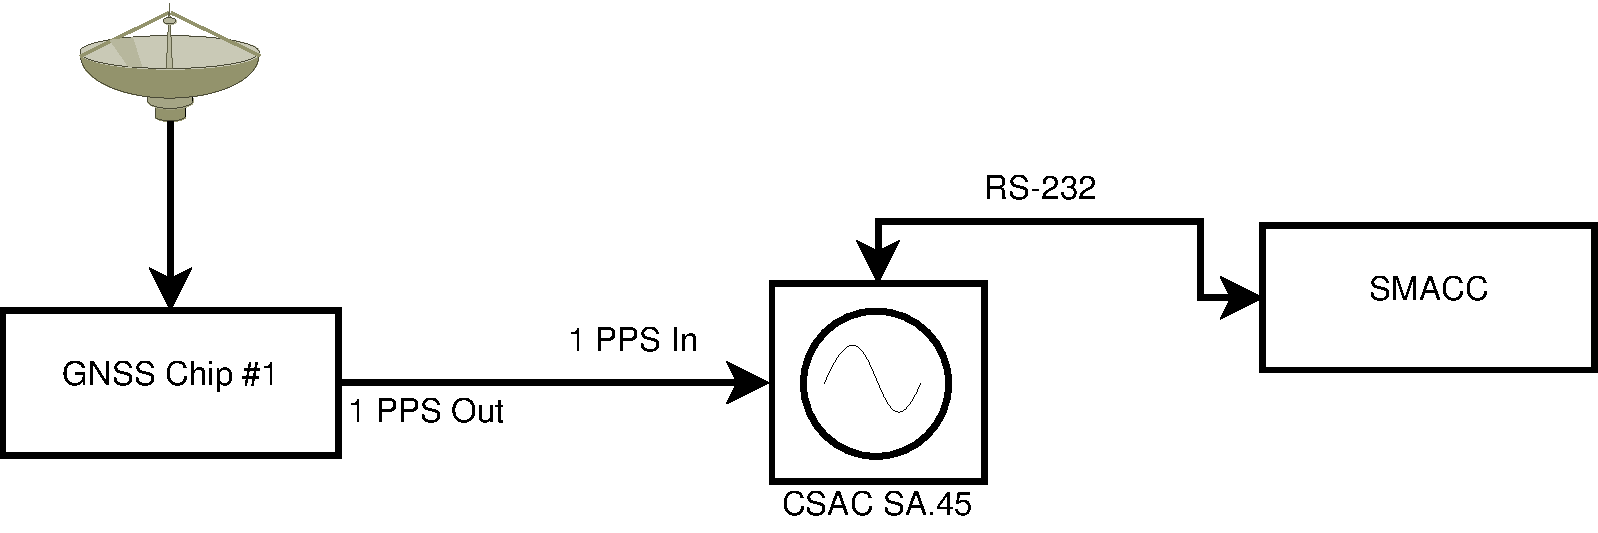
\includegraphics[scale=0.4]{csac_serial.pdf}
   \caption[Block diagram showing the atomic clock connected to a PC]{Block diagram showing the atomic clock connected to a PC}
   \label{csac_filter}
\end{figure}

The SA.45 atomic clock includes a serial interface that enables communication with a PC by using a COM port. As mentioned earlier, our approach relies heavily on the ability to communicate with the atomic clock.
Information can be queried by sending commands to the atomic clock. These commands are explained in table \ref{atomic clock_COMMANDS}. 

\begin{table}[]
  \centering
  \caption{Commands for the SA.45 atomic clock}
  \label{atomic clock_COMMANDS}
    \begin{tabular}{|l|l|l|}
    \hline
    Shortcut          & Description                                        & Command                       \\ \hline
    6                 & Return telemetry headers as comma-delimited string & !6{[}CRLF{]}                  \\ \hline
    \textasciicircum  & Return telemetry as comma-delimited string         & !\textasciicircum  {[}CRLF{]} \\ \hline
    F                 & Adjust frequency                                   & !F?{[}CRLF{]}                 \\ \hline
    M                 & Set operating mode register bits                   & !M?{[}CRLF{]}                 \\ \hline
    S                 & Sync atomic clock 1 PPS to external 1 PPS                  & !S{[}CRLF{]}                  \\ \hline
    D                 & Set 1 PPS disciplining time constant               & !D?{[}CRLF{]}                 \\ \hline
    U                 & Set ultra-low power mode parameters                & !U?{[}CRLF{]}                 \\ \hline
    T                 & Set/report time-of-day                             & !T?{[}CRLF{]}                 \\ \hline
    \end{tabular}
  \caption*{Source: \ref{CSAC_USERGUIDE}}
\end{table}

The Sensor Server communicates with the atomic clock by invoking a script called \texttt{query\_csac.py}. This script can be found in the appendix (\ref{query_csac}). The script takes an argument which it sends to the atomic clock over serial, and prints the respond to the shell which the Sensor Server grabs. In this document, the word \textit{telemetry} gets mentioned quite often in context with the atomic clock. Telemetry can be obtained by querying the atomic clock. The telemetry is a string containing a plethora of information, but we are mainly interested in the following values:

\begin{itemize}
  \item{Phase, the difference between the atomic clock and the external signal signal at 1PPS in.}
  \item{DiscOK, the discipline status.}
  \item{Steer, the frequency adjustment.}
\end{itemize}

Listing \ref{telemetry_string} show an example of telemetry received from the atomic clock. The fourth value from the right, is the \texttt{DisOK}, the fifth is the \texttt{phase} and the \texttt{steer} is the seventh. 

\begin{lstlisting}[caption={Example of a telemetry string received from the atomic clock},label={telemetry_string}]
0,0x0000,1209CS00909,0x0010,4381,0.86,1.573,17.62,0.996,28.26,-24,---,-1,1,1268126502,586969,1.0
\end{lstlisting}

The SA.45 uses a high-resolution phase meter to improve synchronization and to calibrate the frequency of the atomic clock. The phase meter measures the difference in time between the internal 1 PPS signal and the external reference, in our case a GPS receiver. This difference is the \textit{phase} value. The atomic clock uses the phase value and steering algorithms to adjust the frequency of atomic clock's physics package thus simultaneously steering both the phase and frequency to that of the external reference. This is called \textit{disciplining} and is how the \textit{steer} value is computed. The last value, \textit{DiscOK} is simply the status of the 1 PPS disciplining routine \cite{CSAC_USERGUIDE}.

\section{Data structures}
In the C programming language, a "struct" is a complex data type that defines a list of variables to be placed under the structs given name in a block of memory. This makes it possible for multiple variables to be accessed via a single pointer. Before delving deeper into the code base of the sensor server, some crucial and often used structs will be explained in this section.

\subsection{server\_data}
\begin{code}
  \caption{Sample of code taken from \texttt{sensor\_server\_common.h} (appendix \ref{sensor_server_common.h}, line 107) showing the \texttt{server\_data} struct.}
    \begin{minted}
    [
    fontsize=\footnotesize,
    fontfamily=tt,
    linenos=true
    ]
    {c}
    struct server_data {
        int number_of_clients; 
        int number_of_sensors;  
        time_t started;    
        pid_t pid;             
        char version[4]; 
    \end{minted}
  \label{server_data}
\end{code}
The \texttt{server\_data} struct as shown in listing \ref{server_data}, contains information about the server. Some of the of information like the PID, version, and when the server was started, is just information about the server itself. The number of clients and sensors on the other hand, is used to make sure that the server does not allow more connections than it can handle.

\subsection{server\_synchro}\label{server_synchro}
\begin{code}
  \caption{Sample of code taken from \texttt{sensor\_server\_common.h} (appendix \ref{sensor_server_common.h}, line 116) showing the \texttt{server\_synchro} struct}
    \begin{minted}
    [
    fontsize=\footnotesize,
    fontfamily=tt,
    linenos=true
    ]
    {c}
    struct server_synchro {
        sem_t ready_sem;
        sem_t csac_sem;
        sem_t client_list_sem;
        volatile sig_atomic_t done;
    };
    \end{minted}
  \label{server_synchro}
\end{code}
The \texttt{server\_synchro} as shown in listing \ref{server_synchro}, contains "flags" used by synchronization mechanisms (\ref{shared_mem_sem}) that the server and its children processes uses to protect access to shared resources. The \texttt{csac\_sem} is used to control serial access to the atomic clock, making sure that only one request is sent to atomic clock at a time. The \texttt{client\_list\_sem} is used by functions manipulating and reading the client list structure, and the \texttt{ready\_sem} is used by ready check algorithm. See subsection \ref{ready_check_alg} for more about this.

\subsection{command\_code}\label{command_code}
\begin{code}
  \caption{Sample of code taken from \texttt{sensor\_server\_common.h} (appendix \ref{sensor_server_common.h}, line 34) showing the \texttt{command\_code} struct}
    \begin{minted}
    [
    fontsize=\footnotesize,
    fontfamily=tt,
    linenos=true
    ]
    {c}
    struct command_code {
        int code;
        char parameter[MAX_PARAMETER_SIZE];
        int id_parameter;
    };
    \end{minted}
  \label{command_code_listing}
\end{code}
The \texttt{command\_code} struct as shown in listing \ref{command_code_listing}, is used by the parser to more efficiently convey protocol compliant requests and related parameters. See section \ref{parser} for more about the parser.

\subsection{nmea\_container}\label{nmea_cont}
\begin{code}
  \caption{Sample of code taken from \texttt{nmea.h} (appendix \ref{nmea.h}, line 20) showing the \texttt{nmea\_container} struct}
    \begin{minted}
    [
    fontsize=\footnotesize,
    fontfamily=tt,
    linenos=true
    ]
    {c}
    struct nmea_container {
        /* Raw data */
        char raw_gga[SENTENCE_LENGTH];
        char raw_rmc[SENTENCE_LENGTH];

        /* Latitude */
        double lat_current;
        double lat_average;
        double lat_avg_diff;
        double lat_total;
        int lat_disturbed;

        /* Longitude */
        double lon_current;
        double lon_average;
        double lon_avg_diff;
        double lon_total;
        int lon_disturbed;

        /* Altitude */
        double alt_current;
        double alt_average;
        double alt_avg_diff;
        double alt_total;
        int alt_disturbed;

        /* Speed */
        double speed_current;
        double speed_average;
        double speed_avg_diff;
        double speed_total;
        int speed_disturbed;

        /* CHECKSUM */
        int checksum_passed;

        /* COUNTER FOR AVERAGE */
        int n_samples;
    };
    \end{minted}
    \label{nmea_container}
\end{code}

The \texttt{nmea\_container} struct as shown in listing \ref{nmea_container}, is used by the handler (see section \ref{parser_and_handler}) which dissects the NMEA strings and validates them before it fills the respective members of the structs. The purpose of it is just to make it easier for the other parts of the Server to use the NMEA data.

\subsection{list\_head}\label{list_head}
\begin{code}
  \caption{Sample of code taken from \texttt{list.h} (appendix \ref{list}, line 70) showing the \texttt{list\_head} struct}
    \begin{minted}
    [
    fontsize=\footnotesize,
    fontfamily=tt,
    linenos=true
    ]
    {c}
    struct list_head {
      struct list_head *next, *prev;
    };
    \end{minted}
    \label{list_head_listing}
\end{code}

The \texttt{list\_head} struct is shown in listing \ref{list_head_listing}. The fields of the struct is pretty self explanatory. There is a pointer to the previous node and one to the next. One of the members of the \texttt{client\_table\_list} is a struct of type \texttt{list\_head}. This is what makes it possible to traverse the list.

\subsection{transmission\_s}
The \texttt{transmission\_s} struct as show in listing \ref{transmission_struct} is used by the child process forked out by the Server in the server core, communicates with the client. The struct has two members, a file descriptor for the socket and a buffer to store incoming data.

\begin{code}
  \caption{Sample of code taken from \texttt{net.h}(appendix \ref{net.h}) line 31}
    \begin{minted}
    [
    fontsize=\footnotesize,
    fontfamily=tt,
    linenos=true
    ]
    {c}
    struct transmission_s {
        int session_fd;
        char iobuffer[IO_BUFFER_SIZE];
    };
    \end{minted}
    \label{transmission_struct}
\end{code}


\subsection{client\_table\_entry}\label{client_table_entry}
The client\_table\_entry struct is what the name suggests, it's an entry in a list of clients. Every client connected to the server, no matter the purpose, has an entry in the client list. Listing \ref{struct_client_table} shows the complete struct. 

\begin{code}
  \caption{Sample of code taken from \texttt{sensor\_server\_common.h}(appendix \ref{sensor_server_common.h}, line 90) shows the \texttt{client\_table\_entry} struct}
    \begin{minted}
    [
    fontsize=\footnotesize,
    fontfamily=tt,
    linenos=true
    ]
    {c}
    struct client_table_entry {
        struct list_head list; 
        struct transmission_s transmission; 
        struct timeval timeout; 
        struct command_code cm;   
        struct nmea_container nmea;
        struct filters fs;    
        pid_t pid;  
        time_t timestamp;  
        int client_id; 
        int client_type;    
        int ready;  
        int marked_for_kick; 
        char ip[INET_ADDRSTRLEN];
    };
    \end{minted}
    \label{struct_client_table}
\end{code}
Beginning from the top:
\begin{itemize}
  \item \texttt{list\_head list} is used to traverse the linked client list. See \ref{linked_list} for more about the linked list implementation and \ref{list_head} for more about the struct.
  \item \texttt{transmission\_s transmission} is used by the process to network I/O with the connected client.
  \item \texttt{timeval timeout} is defined by the \texttt{sys/time.h} and is used in the Sensor Server implementation to hold a value defining how long a connected client can stay connected without sending any commands to the Server. When the timeout value is exceeded, the client is disconnected. The values are:
  \begin{itemize}
    \item 5 seconds for a Sensor.
    \item 1000 seconds for a Monitor.
    \item 10 seconds for an unidentified client.
  \end{itemize}
  These values are defined in the \texttt{sensor\_server.h} file.
  \item \texttt{command\_code cm} is used by the parser to convey protocol compliant requests. See \ref{command_code} for more.
  \item \texttt{nmea\_container} is used to contain NMEA data in a more convenient way for the filters. See \ref{nmea_cont} for more about the struct, and \ref{nmea_data} for more about NMEA.
  \item \texttt{filters fs} is a struct containing data for the GPS based filters. There is currently only one GPS based filter, the Location and speed filter and it is explained in subsection \ref{gps_filters}.
  \item \texttt{pid\_t pid} is the process ID for the process forked out for the connected client.
  \item \texttt{time\_t timestamp} is time stamp that is stamped every time the Sensor's filter data is processed.
  \item \texttt{client\_id} and \texttt{client\_type} is the client's ID and the client's type, either "SENSOR" or "MONITOR". 
  \item \texttt{ready} is used to indicate that a Sensor has received NMEA data and is ready for filter processing.
  \item \texttt{marked\_for\_kick} is a flag. If it is 1, the client has been marked by a monitor indicating that it should be kicked. The next the client sends data to the Server, the client will be disconnected.
  \item \texttt{char ip} is the connected client's IP address.
\end{itemize}

\section{The Sensor Client}\label{sensor_client}
The sensor client software is a simple program written in C99 whose only task is to relay information read from the GPS receivers. Summed up shortly:
\begin{itemize}
  \item The client software takes two parameters to start, the servers IP and port. If parameters are missing, the program exits.
  \begin{itemize}
    \item Example: \texttt{./sensor\_client -p 10000 -i 192.168.1.5}
  \end{itemize}
  \item Initializes and loads configuration from configuration file. The configuration file includes path to the GPS receiver, the sensors ID number and a binary value for whether or not logging of NMEA should be done as well as path to 
  the log file. If the loading of the configuration file fails, default values are used instead:
  \begin{itemize}
    \item The ID number is chosen at random but within legal limits.
    \item Logging is disabled.
    \item Maximum of server connection attempts are set to 10.
    \item Path to GPS receiver is set to \texttt{/dev/ttyACM0}. This should be the path to the receiver unless another similar device is connected to the computer and given it is a Raspberry Pi running Raspbian.
  \end{itemize}
  \item Establishes communication with GPS receiver, exits if it fails.
  \item Attempts to establish communication with the server, retries for a configurable amount of times at 1 second intervals.
  \item Identifies the client for the server according to protocol.
  \item Reads from the GPS receiver, scans for lines starting with either \texttt{\$GNRMC} or \texttt{\$GNGGA}. When both lines are found, the data is stored in a buffer.
  \item Sends the GPS data to the server according to protocol.
  \item Repeats.
\end{itemize}
Figure \ref{client_call_graph} shows a simplified call graph for the Client.

\begin{figure}\label{client_call_graph}
\centering
  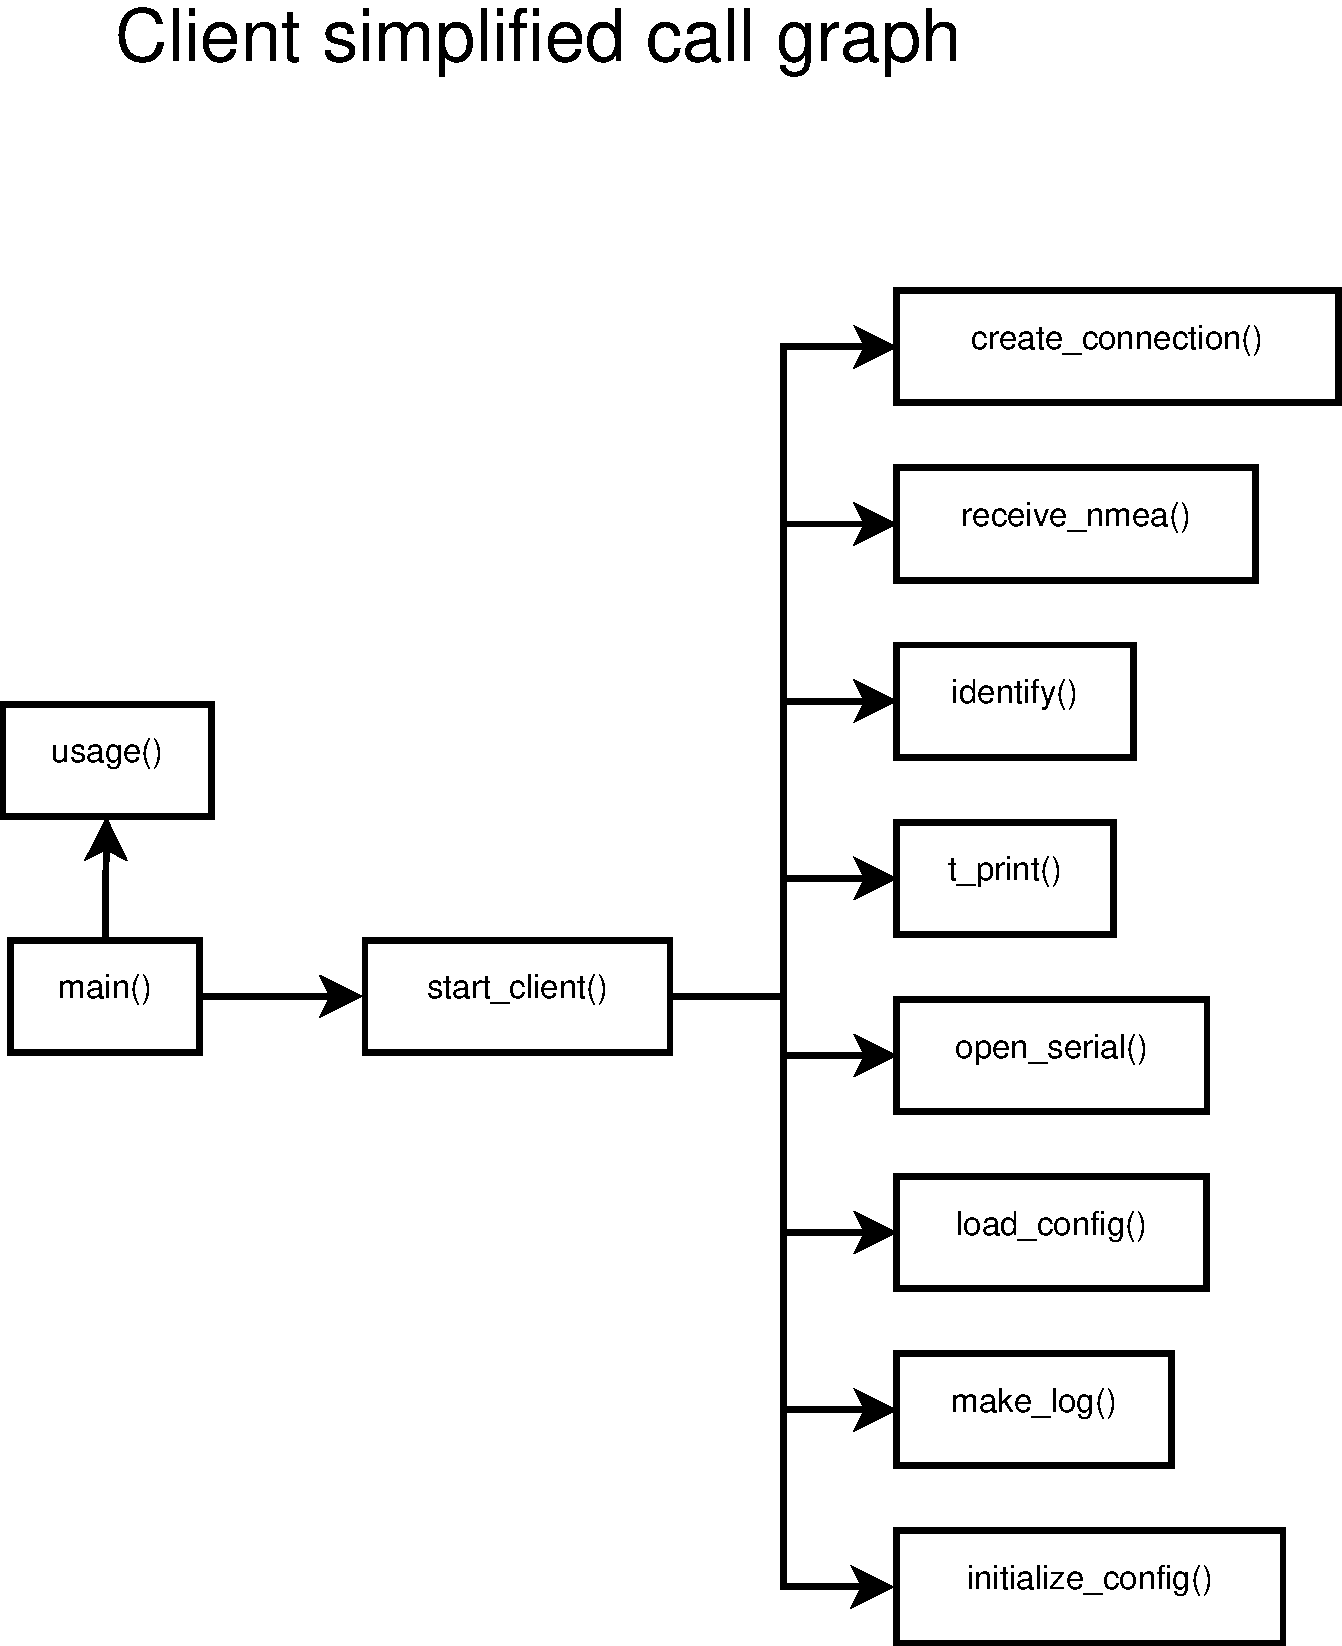
\includegraphics[scale=0.3]{client_call_graph.pdf}
   \caption[Sensor Client simplified call graph]{Simplified call graph for the Sensor Client.}
   \label{client_call_graph}
\end{figure}